% \documentclass[11pt,a4paper,twoside,openright,extrafontsizes]{memoir}

\renewcommand*{\baselinestretch}{1.025}
\isopage
\checkandfixthelayout

\newif\iftdkoneside
\tdkonesidefalse

%%% Local Variables:
%%% mode: latex
%%% TeX-master: "../main"
%%% End:

% We actually use `twoside` in oneside mode to avoid renumbering pages.
\documentclass[11pt,a4paper,twoside,extrafontsizes]{memoir}

\renewcommand*{\baselinestretch}{1.025}
\isopage
\setlrmargins{*}{*}{1}
\checkandfixthelayout

\newif\iftdkoneside
\tdkonesidetrue

%%% Local Variables:
%%% mode: latex
%%% TeX-master: "../main"
%%% End:


% \usepackage{perpage}
% \MakePerPage{footnote}

\usepackage{include/thesis}
\usepackage{enumitem}
\setlist{nolistsep}

\usepackage{rotating}

\usepackage{xcolor,colortbl}

\usepackage{listings}
\lstset{
	basicstyle=\small\ttfamily, % print whole listing small
	keywordstyle=\color{black}\bfseries, % bold black keywords
	identifierstyle=, % nothing happens
	commentstyle=\color{gray},
	showstringspaces=true,
	aboveskip=1em,
	belowskip=0.7em,
	columns=flexible,
	numbers=none,
	backgroundcolor=\color{white},
	extendedchars=false,
	inputencoding=utf8,
	xleftmargin=0em,
	xrightmargin=0em,
	framexleftmargin=0em,
	framextopmargin=0em,
	framexbottommargin=0em,
	frame=none,
	framerule=0pt,
	escapeinside={(*@}{@*)}
}


%
% General
%

\DeclareMathOperator*{\argmin}{arg\,min}
\DeclareMathOperator*{\argmax}{arg\,max}
\newcommand*{\dd}{\mathrm{d}}
\newcommand*{\T}{\mathrm{T}}
\newcommand*{\vecarrow}{}\let\vecarrow\vec
\renewcommand*{\vec}[1]{\bm{\mathrm{#1}}}

%
% Numbers
%

\newcommand*{\RR}{\mathbb{R}} % Reals
\newcommand*{\RRpos}{\RR^{+}} % Positiver reals
\newcommand*{\QQ}{\mathbb{Q}} % Rationals
\newcommand*{\ZZ}{\mathbb{Z}} % Whole numbers
\newcommand*{\NN}{\mathbb{N}} % Naturals
\newcommand*{\NNpos}{\NN^{+}} % Positive whole numbers

%
% Probability
%

\let\Pr\relax
\DeclareMathOperator{\Pr}{\mathbb{P}}
\DeclareMathOperator{\Ex}{\mathbb{E}}

%%% Local Variables:
%%% mode: latex
%%% TeX-master: "../main"
%%% End:


\newcommand*{\bme}{Budapest University of Technology and Economics}
\newcommand*{\vik}{Faculty of Electrical Engineering and Informatics}

\newcommand*{\bmeaut}{Department of Automation and Applied Informatics}

\newcommand*{\vikdoctype}{Master's Thesis}
\newcommand*{\viktdklocation}{Budapest}
\newcommand*{\viktdkyear}{2020}

\newcommand*{\authors}{Authors}
\newcommand*{\advisors}{Supervisors}

\newcommand*{\authori}{Soma Lucz}
\newcommand*{\authorihun}{Lucz Tamás Soma}

\newcommand*{\advisori}{Márk Asztalos}

\title{Developing a graph-based, domain-specific social network}
\newcommand*{\titlepagetitle}{Developing a graph-based,\\domain-specific social network}
\author{\authori}

\hypersetup{
  pdftitle={\thetitle},
  pdfauthor={\theauthor, \advisors: \advisori}
}

%%% Local Variables:
%%% mode: latex
%%% TeX-master: "../main"
%%% End:


\bibliography{bibliography}
\addbibresource{bibliography.bib}

\setlength{\parskip}{8pt}
\setlength{\parindent}{0pt}

\begin{document}

\frontmatter

\cleartorecto
\thispagestyle{empty}

\begin{tikzpicture}[overlay,remember picture]
  \node at (current page.center) [yshift=1cm] {%
    \begin{minipage}{\textwidth}

      \centering

      
\includegraphics[width=7cm]{include/figures/bme_logo}
      \vspace{0.3cm}

      {\textbf \bme} \\
      \vik \\
      \bmeaut \\
      \vspace{3.5cm}

      {\Large \authori \par}
      \vspace{0.5cm}

      {\Huge\sffamily\bfseries \titlepagetitle \par}
      \vspace{1cm}

      {\Large \textsc \vikdoctype \par}
      \vspace{3.5cm}

      {\Large
        {\large \textit \advisors} \\
        \vspace{0.05cm}
        \advisori\par}

      \vspace{1.5cm}
      {\large \viktdklocation, \viktdkyear\par}

    \end{minipage}};
\end{tikzpicture}

\cleardoublepage

%%% Local Variables:
%%% mode: latex
%%% TeX-master: "../main"
%%% End:


\tableofcontents

\cleartorecto
\begin{otherlanguage}{magyar}

  \chapter*{Hallgatói nyilatkozat}
  \phantomsection
  \addcontentsline{toc}{chapter}{Hallgatói nyilatkozat}
  \thispagestyle{plain}

  Alulírott \textbf{\authorihun} szigorló hallgató kijelentem, hogy ezt
  a diplomatervet meg nem engedett segítség nélkül, saját magam
  készítettem, csak a megadott forrásokat (szakirodalom, eszközök stb.)
  használtam fel. Minden olyan részt, melyet szó szerint, vagy azonos
  értelemben, de átfogalmazva más forrásból átvettem, egyértelműen, a
  forrás megadásával megjelöltem.

  Hozzájárulok, hogy a jelen munkám alapadatait (szerző(k), cím, angol
  és magyar nyelvű tartalmi kivonat, készítés éve, konzulens(ek) neve) a
  \textls{BME} \textls{VIK} nyilvánosan hozzáférhető elektronikus
  formában, a munka teljes szövegét pedig az egyetem belső hálózatán
  keresztül (vagy hitelesített felhasználók számára)
  közzétegye. Kijelentem, hogy a benyújtott munka és annak elektronikus
  verziója megegyezik. Dékáni engedéllyel titkosított diplomatervek
  esetén a dolgozat szövege csak 3~év eltelte után válik hozzáférhetővé.

  \vspace{4ex}

  \noindent Kelt: \viktdklocation, 2020. május 31.

  \vspace{-5mm}

  \hfill\begin{minipage}{0.4\linewidth}
    \centering
\includegraphics[width=35mm,clip]{figures/soma-lucz-signature.pdf}\par
    \vspace{-5mm}
    \centering\hbox to \linewidth{\cleaders\hbox{.}\hfil}\par
    \centering\authorihun\par
    \centering s.k.\par
  \end{minipage}

\end{otherlanguage}

%%% Local Variables:
%%% mode: latex
%%% TeX-master: "main"
%%% End:


\begin{otherlanguage}{magyar}

\paragraph*{Kivonat}
\phantomsection
\addcontentsline{toc}{chapter}{Kivonat}
\thispagestyle{plain}

Napjaink globalizált világának működésében kulcsfontosságú szerepet tölt be a diplomácia. Diplomatává válni hosszú folyamat, mely korai elhivatottságot kíván – gyakran középiskolás vagy egyetemista korban, világszervezetek munkájának tanulmányi célú szimulációjában való részvétellel kezdődik egy karrier. \emph{Egy} leendő diplomata karrierjét támogatva nemcsak betekintést nyújthatunk az általa is formált közös jövőnkbe, de hosszú távon annak alakításában is részt vehetünk. \emph{Az összes} leendő diplomata karrierjét tekintve a lehetőségek tárháza határtalan, az ezzel járó felelősség pedig hatalmas.

A \emph{Model United Nations (MUN)} keretrendszerben világszerte évente többszázas nagyságrendben megrendezett konferenciákon résztvevő középiskolás és egyetemista diákok az Egyesült Nemzetek Szervezete (ENSZ) mindennapi munkájának formális szimulációján keresztül tanulhatnak diplomáciáról, nemzetközi kapcsolatokról, világpolitikáról – kockázatmentes, tényekre és információkra alapozott vitakultúrát kultiváló környezetben, gyakran tapasztalt karrierdiplomaták támogatásával.

A világ MUN-közösségének összefogására több szoftveres kísérlet is született. Ezek többnyire egy-egy problémára igyekeznek elszigetelt megoldást adni, így kapcsolatépítésre, konferenciák szakmai szervezésére, illetve rendezvények általános adminisztrációjára eltérő – gyakran házon belüli – szoftverek használatosak. Ezen alkalmazások nem kötik össze a közösség egészét, és nem adnak teljes megoldást az adminisztratív problémákra sem.

Dolgozatomban kifejtem, ahogyan megtervezem, lefejlesztem, és webalkalmazásként publikusan elérhetővé teszem a \emph{Diplomatiq} nevű, MUN-konferenciák szervezésére alkalmas közösségi hálózatot. A \emph{Diplomatiq} hosszú távú célkitűzése az, hogy a diplomaták elsődleges közösségi platformjaként nyújtson integrált megoldást az MUN-világban felmerülő adminisztratív problémákra.

A tervezés és fejlesztés teljes folyamata alatt fókuszban tartottam két alapvető szempontot. Az első szempont, hogy a rendszer „használatra kész” minőségben készüljön el, és később igény szerint bővíthető legyen további közösségi, adminisztratív, illetve valós idejű adatelemzési funkcionalitással. Ennek célja, hogy a szoftver a jövőben az MUN-szcénán kívül valódi diplomáciai alkalmazásokban is helyt tudjon állni. A második szempont – a tárolt személyes adatok, illetve a szoftver leendő alkalmazási lehetőségeinek figyelembe vételével – az, hogy a rendszer már a kezdetektől modern, réteges, kriptográfiai biztosítékokat nyújtó biztonsági architektúrára alapozva készüljön el.

A rendszer tervezése és fejlesztése során a mérnöki szempontokon felül arra is figyelmet fordítottam, hogy a \emph{Diplomatiq}, mint majdani vállalkozás az elvégzett munkámra egyszerűen ráépíthető legyen. A szoftver lefejlesztéséhez és publikációjához szükséges előfizetéseket, szolgáltatásokat és rendszereket mind olyan megfontoltsággal választottam ki és integráltam, mintha egy vállalkozást indítanék el. Dolgozatomban az ezzel kapcsolatban felmerülő adminisztratív és pénzügyi teendők mellett a rendszer egy kezdetleges üzleti modelljéről is beszámolok – kisebb terjedelemben, mérnöki diplomatervről lévén szó.

\end{otherlanguage}

\clearpage

\paragraph*{Abstract}
\phantomsection
\addcontentsline{toc}{chapter}{Abstract}
\thispagestyle{plain}

Diplomacy plays a key role in the operation of today's globalized world. Turning into a diplomat is a long process and involves early dedication — careers often start in high schools or universities, by students taking part in academic simulations of various intergovernmental organizations' work. Supporting \emph{a} prospective diplomat's career not only enables us to peek into the future through them, but in the long run, we can also take part in jointly shaping tomorrow's world. Considering \emph{all} prospective diplomats' careers, the possibilities are endless, and the associated responsibility is immense.

The world of junior diplomats mostly consists of conferences — annually hundreds of them, worldwide — held within the framework of the \emph{Model United Nations (MUN)}. During these events, high school and university students formally simulate the everyday work of the United Nations (UN), which enables them to learn about diplomacy, international relations and world politics — in a risk-free environment, cultivating debates based solely on facts and information. These conferences are often attended by experienced senior diplomats as well, with the goal of supporting and educating the future generation.

There are several software-involved attempts for bringing together the MUN community. Most of these attempts solve one isolated problem of the collective at a time: social networking, organizing the professional part of conferences, and administering the actual events usually involves several different — mostly in-house — software. These applications neither link the community together, nor do they offer a complete solution to administrative problems.

In this thesis I design, implement and publish \emph{Diplomatiq}, a social network software system for diplomats, suitable for organizing MUN conferences. The long-term goal of \emph{Diplomatiq} is to provide an integrated solution for administrative problems in the MUN world, while being the sole professional networking platform for its diplomat users.

During the whole process of the design and implementation, I focused on two key points. The first point is that the system should be implemented in production-grade quality, and it should be easily extendable with further social, administrative, and real-time data analytics features as needed. The goal of this is to enable the system to cover the needs of real-world diplomatic applications as well, outside the MUN scene. The second point — considering the stored personal information, and the prospective future applications — is that the system should be implemented upon a modern, layered security architecture, which provides cryptographic assurances in terms of application and data security.

Besides engineering aspects, I also paid attention to being able to build \emph{Diplomatiq} as a prospective company upon my work. Subscriptions, services and systems needed for the implementation and publication were chosen and integrated with the same amount of consideration as I was starting company. In this thesis I present the related administrative and financial aspects of this too, as well as a primitive business model — briefly only, this being an engineering thesis.

%%% Local Variables:
%%% mode: latex
%%% TeX-master: "main"
%%% End:


\mainmatter

\chapter{Introduction}
\label{chapter:introduction}

\section{Context}

Diplomacy is the art and practice of conducting negotiations between nations and nationwide entities~\cite{diplomacymerriamwebster}. It is a complex system, where involved parties like governments and NGOs\footnote{non-governmental organizations} engage in formal discussions, aspiring to \emph{peacefully} influence the status quo of international relations along their interests. Parties are represented by selected, often professionally trained career diplomats, forming a diplomatic delegation.

Besides diplomacy, there are other tools for leveraging international relations. This set of tools, tactics and strategies is collectively known as foreign policy, and is usually directed by political leaders~\cite{foreignpolicybritannica}. Foreign policy is often collated with diplomacy as a synonym, but the two are not identical. Diplomacy is a key instrument of foreign policy, and foreign policy is a superset of diplomacy. In order to achieve the objectives of a nation, tools of foreign policy can include espionage, threats, sabotages, wars, and other means of violence, as well as diplomacy.

Throughout this thesis, I consider diplomacy as the nonviolent elements of foreign policy: the system, methods and infrastructure of governments and NGOs peacefully interacting with each other, in order to influence international relations along their own objectives. Although most diplomacy materializes in confidence between parties, this thesis exists in the context of publicly conducted diplomacy, more narrowly in the context of the United Nations (UN), which — having 193 sovereign member states — is the largest intergovernmental organization in the world~\cite{unmembers}.

Being a powerful diplomat requires experience in various fields. Diplomats need strong organizational and leadership skills, as well as proficiency in written and oral communication for efficient negotiations. They must be able to stay rational and decisive in stressful situations, besides the capacity to quickly process and integrate information into their decisions~\cite{fsicapabilities}. These skills can be developed in specialized educational institutes, usually offering graduate programs~\cite{usdoddiplomattrainings}.

Apart from professional programs designed to train already graduated career diplomats, there are other ways to gain diplomatic experience. One of these is taking part in academic simulations of the United Nations' everyday work. For high school and university students, the Model United Nations (MUN) framework\footnote{The concept of Model United Nations is detailed in \Cref{section:munframework}.} offers hundreds of independent conferences annually, worldwide~\cite{mymunconferencelist}. On these few-day-long events, participants become diplomatic delegates. They are placed in UN-like committees and assigned countries to represent. Assignments are published in advance, along with the topics the committees will discuss. This enables delegates to perform research and develop their positions before the conference, usually staying true to the actual position of their represented country. During the conference, delegates discuss their positions in the committees, conforming to the formalities of the real-world United Nations, like western business attire and the method of moderated formal debate. By the end of the conference, each committee produces a formal, UN-like \emph{resolution}: a document summarizing the results of their debate and formulating measures for resolving the international issues presented to the committee.

\section{Problem statement and requirements}

Since even a medium-sized conference welcomes hundreds of international students, who need housing, meals, conference accessories like badges and placards, topics to debate, merchandise, and afterwork entertainment, an MUN conference is a heavy organizational burden, requiring months of preparation. Most conferences are driven, prepared, implemented, and executed by voluntary, unpaid students of an educational institution — a high school or a university —, as an extracurricular activity, with additional help of their teachers. Professional event planners, IT and data administrators or other experts are usually not involved. Also, the staff rotates relatively fast as organizing students graduate and leave the institution, making it harder to reuse last year's experience.

Although in general conferences are self-sustaining by making use of participation fees, the execution quality of the event depends on the creativity, enthusiasm, and personal experience of the students at the top of the organizational hierarchy, rather than a solid financial basis. This results in the lack of ability to build modern, automated organizational tools, which ultimately causes data management to be cumbersome and insecure — even though the major part of the organizational work is indeed data management and batch processing. A software system offered as a rationally priced service, tailored to the administrative needs of MUN conferences could greatly reduce this organizational burden by providing easy-to-use data management features.

Aside from the organizational concerns, MUN conferences provide outstanding networking opportunities to both the participants and the organizers. Participants working themselves towards a diplomatic career can substantially benefit from building global acquaintances among their future colleagues. Experienced career diplomats attending MUN conferences as guests can open doors for prospective diplomats which no education can. Professional networking among future and current diplomats can be supported and facilitated well by a suitable software system.

Inspecting current solutions, there is no software system on the internet, which solves the administrative problems of MUN conferences, while making use of the great networking potential of the MUN framework. Implementing such a system would appreciably further global diplomacy in the long run.

\section{Objectives and contributions}

In this thesis I present \emph{Diplomatiq}, a social network software system for diplomats, suitable for organizing MUN conferences. On the one hand, I will refer as \emph{Diplomatiq} to the software system itself, and on the other hand, to the prospective company conducting the maintenance, marketing and sales operations of the software system. Outside the context of this thesis, the social network is the first step of a long-term plan involving global consumption of public data, for producing real-time diplomatic prognoses and analyses.

My first objective was to design and implement Diplomatiq on a solid, production-grade foundation, with a minimal feature set, which can be extended with further social networking, administrative, and real-time data analytics capabilities as needed. Considering the sensitive personal information stored in the system, the prospective applications of Diplomatiq, and my deep interest in cryptography and computer security, my second objective was to build the system upon a modern, layered security architecture, which provides cryptographic assurances in terms of application and data security.

My contributions include the following:

\begin{itemize}
\item I designed, built, secured and paid a company-level production infrastructure for the development, publication and maintenance of Diplomatiq, including several kinds of supportive infrastructure.
\item I designed, implemented and published the Diplomatiq social network software system as a client-server application, using graph database technologies.
\item I developed several supportive libraries outside the Diplomatiq software along the way. I published the built artefacts of these libraries with documentation, for free use in the open-source community.
\item I published the source code of all my contributions as separate open-source projects, centralized under one project organization, called Diplomatiq.
\end{itemize}

\section{Structure of this thesis}

The thesis is structured as follows.

\begin{itemize}
\item \emph{\Cref{chapter:preliminaries}} summarizes the preliminary knowledge needed for a high-level understanding of this thesis. It details the concept of Model United Nations and my personal experience with MUN. It also defines the idea of a social network. Then it introduces graph database technologies, focusing on the property graph data model and the Neo4j graph database.
\item \emph{\Cref{chapter:relatedwork}} gives examples for domain-specific social networks, and presents existing software solutions for the MUN community.
\item \emph{\Cref{chapter:infrastructure}} describes my approach of building and securing a production-grade infrastructure supporting the development and public operation of Diplomatiq, the social network.
\item \emph{\Cref{chapter:libraries}} gives an overview about the produced supportive libraries. It unfolds the reasons of their existence, as well as their features and implementation details.
\item \emph{\Cref{chapter:diplomatiq}} demonstrates the Diplomatiq social network application. It discloses the chosen technologies and client-server architecture, its features and development methods, and implementation details.
\item \emph{\Cref{chapter:security}} reveals the applied cryptographic and other security measures I built into Diplomatiq, in order to protect user and system data from unauthorized access, from the API to the database level.
\item \emph{\Cref{chapter:business}} gives a brief insight into the business considerations of Diplomatiq.
\item \emph{\Cref{chapter:conclusion}} concludes the thesis and presents possible future directions.
\end{itemize}

\chapter{Preliminaries}
\label{chapter:preliminaries}

This chapter summarizes the preliminary knowledge needed for a high-level understanding of this thesis. It details the concept of Model United Nations and my personal experience with MUN. It also defines the idea of a social network. Then it introduces graph database technologies, focusing on the property graph data model and the Neo4j graph database.

\section{The Model United Nations framework}
\label{section:munframework}

\subsection{Introduction}

The Model United Nations (MUN) framework is an academic simulation of the everyday operation of the United Nations (UN). It is typically an extra-curricular activity materializing as annual, few-day-long conferences organized by students of high schools or universities. Participants welcomed from all over the world take on the roles of assigned nations' UN delegates, forming diplomatic delegations with their peers. There are hundreds of such conferences taking place every year~\cite{mymunconferencelist}. While a medium-size conference has a few hundreds of participants and another few hundreds of organizers, the current largest Model UN conference — The Hague International Model United Nations (THIMUN) — attracts over 3,200 students from around 200 schools, from more than 100 different countries~\cite{thimunabout}.

Delegates are placed in UN-like committees, where they discuss topics related to international issues and conflicts by the methods of moderated formal debate. The conduct of the debates and the conference is specified in the \emph{Rules of Procedure}, a conference-specific, formal regulation derived from a similar document of the United Nations~\cite{unmunrop}. The result of the debate is a UN-like \emph{resolution}: a formal document expressing the opinion or will of a committee. Resolutions are generally recommendations, but in some cases — like in case of a resolution adopted by the Security Council: the UN body with \textquote{primary responsibility for the maintenance of international peace and security}~\cite{uncharter} — the adopted resolution is legally binding for all member states. Although MUN resolutions are of course never legally binding, larger MUN conferences like THIMUN forward their adopted resolutions to the UN. These forwarded MUN resolutions are occasionally formulated into real-world UN resolutions after further debate and amendments.

The country and committee assignments are known in advance, which enables delegates to perform research and develop their positions before the conference. Students usually build their stances upon the actual standpoints of the countries they represent, but this is not a requirement. Since usually all positions of a given country's diplomatic delegation is assigned to students arriving from the same school, delegates representing the same country can construct complex nationwide strategies across different committees by cooperating with each other in advance.

The larger a conference is, the more possibilities it has regarding the simulation of the actual workings of the UN, or — as the community reinvents itself — even other intergovernmental bodies, like subsidiaries of the European Union. Even though the UN has only 193 member states~\cite{unmembers}, simultaneously simulating the whole operation of the six main organs\footnote{The six main organs of the UN are: the General Assembly with several subsidiary boards, commissions, committees, councils, panels, working groups and others~\cite{gasubsidiaries}; the Security Council; the Economic and Social Council; the Trusteeship Council; the International Court of Justice; and the Secretariat~\cite{unmainorgans}.}, and the Secretariat of the UN requires much more participants.

\subsection{History}

The history of Model United Nations dates back to the early 20\textsuperscript{th} century. The first similar event is believed to be held in November 1921 by the Oxford International Assembly~\cite{historyofthefirstmun}. It was based on the operation of the League of Nations, the first worldwide intergovernmental organization founded by the Allied powers after the First World War to maintain world peace. Although the League of Nations was formally disbanded in 1946 and its powers were transferred to the United Nations established in 1945, the organization marks an important milestone of intergovernmental cooperation~\cite{leagueofnationsbritannica}.

The first well-documented Model League of Nations conference was organized by the Harvard International Assembly in 1923. It featured the same basic characteristics that modern MUN conferences have: organized by an academic institution, moderated formal debate about international conflicts in committees, and resolutions adopted as the result of the work conducted on the conference~\cite{historyofthefirstmun}.

The era of Model United Nations started in the 1950s with the establishment of the first high school MUN, Berkeley Model United Nations in 1952, and two other MUNs founded by Harvard University: Harvard Model United Nations in 1953 and Harvard National Model United Nations in 1954. The founding of The Hague International Model United Nations in 1968 led to the global expansion of high school MUN conferences~\cite{top10eventsofmun}. THIMUN was the first MUN in Europe, and is today's largest MUN conference~\cite{thimunabout}. In 1991, the Harvard WorldMUN, a university level MUN rapidly accelerated the spread of university-level MUN. In 2007, the actuation of the BestDelegate.com portal significantly increased the online existence of MUN, providing research and preparatory resources for delegates attending MUN conferences. Founding of MyMUN, an MUN-specific registration and administration system, and MUNPlanet\footnote{At the time of writing this thesis, the website of MUNPlanet~\cite{munplanetwebsite} is not reachable, and its Facebook page~\cite{munplanetfacebook} having more than 150,000 followers received its last update in June 2019.}, an MUN-specific social and knowledge-sharing network furthered the presence of Model United Nations on the Internet~\cite{top10eventsofmun}.

\subsection{MUN in numbers}

I have not found any databases, publications, or studies, which would yield satisfactory statistics about Model United Nations. However, according to several portals, websites and Facebook-pages, we can make assumptions about the worldwide spread of MUN.

\subsubsection{Conferences}

At the time of writing this thesis, MyMUN lists 2,457 conferences from December 2012 until today~\cite{mymunconferencelist}. Calculating with roughly 8 years, and with the broad simplification that there were an equal number of conferences organized every year, there are annually more than 300 conferences worldwide, at least based on solely the data of MyMUN. Considering that MyMUN covers only a small fraction of all MUNs in the world, the number of annual MUN conferences likely goes well into the order of thousands.

\subsubsection{Participants}

MyMUN claims having over 100,000 registered members and over 900,000 yearly visitors~\cite{mymunwebsite}. The Facebook page of MUNPlanet~\cite{munplanetfacebook} has over 150,000 followers. According to a 2007 calculation~\cite{howbigismun}, there are 180,000 MUN participants in the United States only. The BestDelegate.com portal is used by over 750,000 people worldwide~\cite{bestdelegate-about}. Considering the numbers above and MUN's increasing popularity, I would assume that millions of unique students attend Model United Nations conferences every year.

\subsection{Networking within Model United Nations}

MUN conferences offer a number of networking opportunities. First of all, delegates attend committee sessions, where they debate international issues, cooperate in producing resolutions, and leverage simulated international relations along their represented countries' best interests. Therefore the main contact point among them is work: they get to know fellow delegates by observing their leadership, public speaking, and negotiation skills in a competitive field. Committee and lunch breaks enable them to further their acquaintances during the day either professionally or personally.

Professional diplomats attending conferences as guests can also take part in committee sessions as observers, or as actual delegates or chairpersons, but they are more likely to attend the official ceremonies or soirées\footnote{elegant evening party, usually with snacks and drinks}. This way, delegates can interact with professional diplomats without unnecessary formalities of real-world diplomacy. Career diplomats are renowned to have appreciable social skills~\cite{fsicapabilities}, which in this setting helps further loosing the mood, and leads to fruitful conversations between generations.

Besides professional programs like debate sessions and official ceremonies, conferences provide a number of other opportunities for delegates to get acquainted with each other. Events like organized sightseeings and afterwork parties allows building informal bounds alongside professional ones.

Aside from maintaining virtual friendships, members of the MUN community often harmonize their conference participations to meet with their foreign acquaintances. Since there is no suitable networking platform for this scenario, participants from different countries usually keep connected and communicate via general social networks, like Facebook. Due to the lack of Facebook's MUN-specific capabilities, a large part of the networking effect is lost, as delegates are not given automated suggestions on which conferences to attend based neither on their circle of friends, nor on their previous Model UN experience.

\subsection{Administration of a Model United Nations conference}

The general administration of a conference can be divided to two distinct parts. The \emph{professional division} involves administrative tasks related to the Model United Nations framework itself: composing the discussed topics, assigning countries and committees to members of delegations, conducting the actual debates and formal ceremonies, and every other features associated with diplomacy. The professional division encompasses everything inside the simulation, where the participants are in their diplomatic roles. The \emph{organizational division} covers the real-world event outside the simulation: travel and hotel arrangements, meals, conference accessories, merchandise, entertainment, among others. According to my personal organizational experience to be detailed in \Cref{section:personalexperience}, the two divisions are separate responsibilities requiring completely different experience, and thus best to be kept as isolated as possible.

Similarly to the United Nations, the chief administrative officer of an MUN conference is usually the \emph{Secretary-General}, responsible for organizing, administering and conducting the conference. In case of the aforementioned two-division administrative approach, the Secretary-General is responsible only for the professional division of the conference, and reports to the \emph{Conference Manager} or \emph{Project Manager}, who leads the organizational division, and is responsible for the entire conference. Henceforth I refer to the organizational and professional divisions together as management.

In the following sections I detail the procedure of organizing a medium-size, high school-level MUN conference with the two-division administrative approach, broken down to distinct, preemptive phases. Most of the following is based on my personal experience, but it also contains parts I learned from event planners or other Model United Nations conference organizers.

\subsubsection{Preliminary arrangements}

Once the management of the previous year's session agreed upon their successors, the new management starts negotiations with the headmaster of the organizing school. They settle the dates for the conference, discuss necessary resources the school can provide, and start or continue securing external locations\footnote{External locations are often needed to be secured years in advance.} for larger conference ceremonies involving all participants, which the school usually cannot host.

After the initial negotiations, the management announces the conference's subsequent session in the host school with its date and vacancies in the organizational structure, and starts coordinating interviews with eventual applicants wishing to take part in organizing the conference.

\subsubsection{Participants' application to the conference}

After the professional division agreed on the UN bodies to be simulated, they publish preliminary committee assignments with high-level topics on the conference's website or Facebook page. As the management opens the application for participants, delegations and individual delegates apply to the conference specifying their preferences of country and committee assignments. Since high school students rarely travel abroad alone, a delegation is usually accompanied by a couple of teachers of the applicants' school. The accompanying teachers are recorded into the registration system as well as the students.

The application procedure comes with significant paperwork. The management consisting of junior members usually lack the experience and resources for efficiently and securely processing sensitive personal information\footnote{Registration data usually includes the applicant's name, birthdate, email address, phone number, and home address. It is also common to require the applicant's social security number or even the serial number of their passport for speeding up any immigration-related checks and administration.} of hundreds or thousands of applicants, and a school's IT division cannot be expected to be prepared for developing a suitable system either. Thus it is common that the registration is implemented with a simple online form populating insecure spreadsheets, or a primitive in-house application often making data management only more complex. Ready-to-use software like MyMUN are often not customizable enough to be useful for conferences generally requiring somewhat tailored solutions, which leads to the usage of multiple different applications. This can cause more pain than gain by requiring manual data maintenance in unintegrated systems.

\subsubsection{Accepting or rejecting applications \& finalizing country and committee assignments}

Following the closure of the application procedure, the management decides about the acceptance or rejection of prospective participants. As applicants usually register as part of their school's delegation consisting of multiple delegates, it is common that the application of an entire delegation gets accepted or rejected together.

Whether to accept a delegation's application to the conference is decided by considering various factors: these can include the delegation's level of expertise — often with regards to the reputation of previously attended conferences —, the ability of fulfilling their preferences of represented countries provided at registration, and aspects of diversity, among others. In case of more mature conferences, committees are often classified by their members' expected level of MUN experience. A beginner delegate taking a seat in an expert-level committee is inexpedient, as it sets back the efficiency of the debate, or vice versa, it prevents the delegate from staying on their learning curve.

Accepting delegations happens in the interest of filling committee seats — predefined seats of countries represented in committees — in the best possible combination with regards to expertise, personal preference, diversity, and the prospective efficiency of the committee's work. Creating the final assignments of delegations and country-committee pairs can be challenging if done manually, considering the volume of input data, and the factors needed to be taken into account. Most conferences do the entire assignment process by hand, in spreadsheets, along a malleable set of priorities. This usually means playing with the synthesis of the committees until all delegations desired by the management can be offered a place to the conference close to their preferences.

This process can be automated, if the management composes a definitive set of priorities on how to assign already fixed committee seats — country-committee pairs — to the applied delegates as individuals. The problem of creating the assignments with the aforementioned conditions is a fundamental problem of combinatorial optimization: it is called \emph{maximum weighted bipartite matching} or \emph{assignment problem}~\cite{ropi}. Mathematically speaking, we are looking for the maximum-size matching in a weighted bipartite graph, where the sum of the edges' weight is maximal. One part of the graph is the set of applicants, and the other part is the set of committee seats. The edges between parts represent possible assignments, and their weights are \textquote{goodness} values based on assignment priorities composed by the management. Since this approach does not cover the possible requirement of all delegates from the same school needing to represent the same country, it is not always satisfactory.

If same-school students need to represent the same country, the process can still be automated with maximum weighted bipartite matching, but with an additional constraint: the management must restrict the application to fixed-size delegations. In this case, a participant school's fixed-size delegation applies to the conference as a whole, specifying their preferences from the set of same-size delegations of represented countries on the conference. This way, the bipartite graph's two parts consist of school delegations applied and country delegations represented on the conference. An edge between the two parts means that the two kinds of delegation are of the same size, so they can be assigned to each other. The weight of an edge is the same \textquote{goodness} value based on assignment priorities composed by the management. This approach needs a second application step: after applied school delegations were assigned country delegations represented on the conference, the applicants of the delegations need to distribute the assigned committee seats among themselves.

\subsubsection{Payment}

The participation fees are collected after the registration, generally in multiple parts. International bank transfers executed by students and teachers usually renders the work of the conference's accounting department challenging, as it is often difficult to identify which delegation made which payment. Due to the general lack of integrated payment solutions in the MUN scene, conferences often face a heavy burden of financial paperwork.

A conference management system with integrated payment processing and accounting features could solve these organizational problems. It would also provide a cleaner experience to the participants: they could pay instantly and individually, without the troubles of needing to transfer the money in groups, as whole delegations.

\subsubsection{Travel, hotel, meal and other arrangements for participants}

With the closure of the acceptance and the assignments procedure, the final list of students and their accompanying teachers taking part on the conference becomes available, and the management can start working on participants' personalized experience. Though habits differ, most conferences offer various convenience services for additional fee, such as transport within the city, accomodation, meal arrangements, and tailored sightseeings or other entertainment programs. This causes lots of additional paperwork with regards to delegation's arrival and departure dates, hotel or other kinds of accomodation preferences, and several kinds of meal allergies and eating habits\footnote{Since participants arrive from all around the world, conferences generally offer multiple types of menus respecting various cultures and allergies.}.

Similarly to the registration, most of the organizational paperwork in connection with convenience services is done manually. A capable software system possessing all information of a delegation's precise schedule, as well as their hotel, meal and entertainment preferences, could automate all this paperwork away. This would allow the management to focus on the quality of the provided services instead of administration. Also, it would open additional financial possibilities. Following preliminary arrangements between the conference management and hotels or other service providers, the applicants could purchase their necessities by selecting them from a list of integrated services during the application procedure. This would endorse further financial cooperation between parties — the conference, the company providing conference management software, and the service providers —, while providing a simple, one-step payment flow for the participants.

\subsubsection{Personalized conference accessories}

MUN conferences formally require participant students, teachers, and all other conference personnel to possess various personalized items. Every person — participants, guests, organizers, staff — should wear an official, conference-issued badge during all events of the conference. The badge usually describes the person's name and title — either a diplomatic one within the simulation in case of participants or guests, or an organizational one in case of organizers or members of staff. Participant delegates, chairpersons, teachers, guests and everyone else attending committee sessions should have official, conference-issued placards in front of them, describing their represented country or position within the committee. Placards are used for voting in larger committees, as well as for identifying delegates from the distance.

Producing hundreds or thousands of personalized items without experience and proper tools can be time-consuming. Management teams generally do not possess neither the experience nor the tools, which leads to hours or days of manual work of creating personalized elements, one by one. Besides being error-prone, this process consumes valuable organizational resources. A capable software possessing all necessary information about participants and organizers could automate away this manual work.

\subsubsection{Conducting the conference}

Following a half-year or longer period consisting of planning and preparation only, conducting the conference itself is usually not a real challenge. Administratively, the management needs to record whether arrived delegations signed in, and received their conference packages, but from the opening ceremony through the committee sessions and parties to the closing ceremony, the conference generally goes by itself, being already scheduled well.

\subsubsection{Processing and storing resolutions and conference data}

Few MUN conferences pay attention to the collection and storage of conference data. As management teams usually lack the resources and experience for keeping digital or paper-based documents, produced resolutions and other conference data is generally not preserved. A capable conference management system could offer solutions for this: with online resolution editing and automated video recording features, the management would not even need to collect conference data, because all of it would immediately be saved in the conference management software's permanent online database.

\subsection{Personal experience: Budapest International Model United Nations}
\label{section:personalexperience}

The previous section's points are mostly based on my personal organizational experience regarding Model United Nations. My former high school, Eötvös József Gimnázium, located in the 5\textsuperscript{th} district of Budapest, first organized \emph{Budapest International Model United Nations (BIMUN)} in 2011 April\footnote{The school has organized BIMUN conferences every year since then. Unfortunately, the tenth anniversary session of BIMUN, which would have been held this year, got cancelled due to the COVID-19 pandemic.}. BIMUN was among the first large-scale international MUN conferences in Hungary~\cite{bimunhistory}. Previously I had attended several foreign MUN conferences, and I was looking forward to take part in the organizational process of an international conference welcoming hundreds of students and diplomatic guests. Over the course of 6 years, I fulfilled several positions: I was a photographer, team lead, deputy Secretary-General, and part of the chief management as an executive advisor.

\section{Social networks}

\subsection{Introduction}

The term social network is used in social sciences, denoting a network of linked individuals or organizations, connected by social relations and interactions~\cite{Borgatti892}. This thesis focuses on another aspect of social networks: online software providing networking, information sharing and messaging features for participating individuals or organizations. The two interpretations are related: users of a social network software form a social network in the scientific sense, and a social network can be loaded into a social network software for analysing patterns, or simply for facilitating interactions among social actors. Analysing social networks can be useful in various fields, including organizational studies and information sciences, and also in diplomacy~\cite{networkdiplomacy}.

\subsection{Connection with graph theory}

Since social networks essentially are connected entities, an obvious choice for modeling such networks is using graphs, where vertices are individuals or organizations, and edges are connections or interactions between them. This way networks are easier to visualize and understand~\cite{socialnetworkvisualization}, and graph algorithms are useful for various kinds of analyses~\cite{socialnetworkanalysis}. By using different kinds of edges in the same graph, several kinds of connections can be represented within the same entity set, allowing to build a multi-dimensional model of the network. This can lead to deeper insight into network structure.

\subsection{Social networking services}

In this thesis I consider social networking services as social networks with associated features the network members can utilize, offered as mass-available services on the Internet. Besides the core networking activity of building relationships within the network itself, associated features can include messaging, information sharing, and collaborational functionality, among others. Usually the goal of a social network is to provide the possibility of interaction among participants, beyond actual in-person interactions. This enables individuals to connect with others regardless of physical distance.

Social networks can be categorized into four main types~\cite{thelwall2009}, but with regards to the focus this thesis, I divide the set of social networks into two parts.

\begin{itemize}
\item \emph{Generic social networks} have no special characteristics or determined target audience: they offer a set of generic features for people to build and maintain virtual relationships with or without personal acquaintance.
\item \emph{Domain-specific social networks} have a determined target audience: they offer specialized features for members of the target audience in line with specific goals of usage in a given domain.
\end{itemize}

Real-world examples for generic social networks include Facebook~\cite{aboutfacebook}, Twitter~\cite{abouttwitter}, and Instagram~\cite{aboutinstagram}. Facebook is the biggest social networking service in the world, having approximately 2.6 billion monthly active users~\cite{facebook2020q1report}. It has several kinds of features for sharing ideas, photos, live or recorded videos, for connecting with friends, and for informing others in various ways. It also offers basic event-handling capabilities for facilitating in-person social interactions. Facebook's business model is based on targeted, personalized advertisement: it offers free features for users, who receive ads in their newsfeed and on other interfaces~\cite{fb-business-model}. The platform has been continuously learning user preferences, and personalizes ads according to the user's assumed needs. Facebook's financial income is mostly based on the fees paid by businesses for publishing and targeting their advertisements in various applications of the social networking platform.

Twitter is a social network gained popularity by providing microblogging features. Users can publish short \textquote{tweets}: posts with at most 280 characters\footnote{Until 2017 November, the maximum length of a tweet was 140 characters~\cite{twitter-doubling-character-limit}.}. It is asymmetric, meaning users can follow other users instead of needing to get virtually acquainted — although for private profiles, users need to be explicitly granted access. Twitter has approximately 166 million daily active users~\cite{twitter2020q1report}, and builds its revenue upon advertising and data licensing~\cite{twitter-business-model}.

Instagram is a social network primarily used for sharing photographs capturing important moments. Despite the fact it is mainly used for image sharing, Instagram can still be regarded as a generic social network, because it is not to be interpreted within a specific domain, and has no determined target audience. Similarly to Twitter, it is asymmetric, but also has private profiles. Instagram was acquired by Facebook in 2012~\cite{facebookacquiresinstagram}, and shares the same basic characteristics regarding its business model: users receive sponsored posts and stories as personalized advertisements.

Diplomatiq is a domain-specific social network. Its domain is diplomacy, its target audience is the set of junior and senior diplomats and other people working in diplomacy, and its specialized features — currently a very basic set of functionalities — include organizing MUN conferences. Broadening the capabilities of Diplomatiq will expectedly not alter its domain-specificity. Further domain-specific social networks are mentioned in \Cref{chapter:relatedwork}.

\section{Graph database technologies}

Graphs are mathematically defined data structures being broadly used in several fields of computer science. Recent technologies and implementations made possible for developers to easily embed graph data models into their applications. There are numerous real-world scenarios which can be represented more efficiently as graphs (\emph{nodes} connected to each other by \emph{edges}), than with the traditional, relational approach.

Graph databases are NoSQL databases, which store data in graphs instead of the traditional, table-based approach\footnote{The underlying data storage methods vary. There are graph databases which store graph data in relational tables, introducing another layer of abstraction between the stored physical data and the database.}. In graph databases, a relationship represented as an edge in the graph is a \textquote{first-class} entity, and has the same basic storage characteristics as a node. Relationships are directly linked to entities, and therefore entities are directly linked to each other via relationships. This allows the querying of related entities to be fast, since the process does not involve lookups.

\subsection{The property graph data model}

It is common to define graphs as a set of objects, in which some object pairs are connected to each other. In this model, an object is called \emph{vertex} or \emph{node} or \emph{point}, and a connection between two \emph{vertices} is called \emph{edge} or \emph{relation}. Connections can be detailed further by specifying their directionality, also they can be \emph{labeled} to define them even more. Similarly labeling vertices leads to the model of \emph{typed graphs}. If we assign properties to the nodes or relations, we get the model of \emph{property graphs}. Properties, as shown in \Cref{fig:property-graph}, are usually key-value pairs in the format of \lstinline{key = `value'}. Generally, keys are strings, and values represent common data types like string, integer, float, etc.

\begin{figure}[!htb]
    \centering
    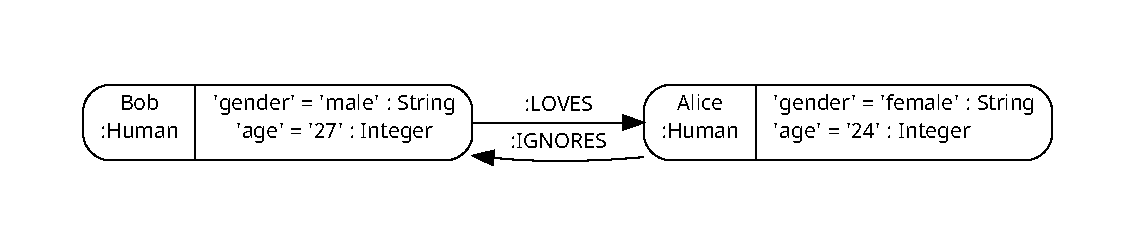
\includegraphics[width=\textwidth, trim=12mm 12mm 12mm 12mm,clip]{figures/property-graph.pdf}
    \caption{Two people's relationship modeled with a property graph}
    \label{fig:property-graph}
\end{figure}

\subsection{Neo4j}

Among a handful of graph database vendors~\cite{graph-dbs}, Neo Technology's Neo4j is the most popular one~\cite{graph-dbs-raking}. It features full ACID-compliance upon a pure graph data model, contrary to other vendors' multi-model approaches. Besides Neo Technology, Neo4j is backed by the open-source community as well~\cite{neo4j-github}. There are two variants: \emph{Community Edition} and \emph{Enterprise Edition} with an extended feature set~\cite{neo4j-licensing}. Neo4j also offers a program tailored to startup companies~\cite{neo4j-startup-program}. With the help of this startup program, companies can build their applications on the Enterprise Edition of the Neo4j platform, free of charge\footnote{Certain limitations apply: the company must have at most 50 employees and at most \$3 million annual revenue, among others~\cite{neo4j-startup-program}.}.

\subsection{Cypher}

Cypher is a query language developed especially for graph databases by Neo Technology~\cite{neo4j-cypher}. \Cref{fig:cypher-intro} shows that the language uses a sort of ASCII-art to represent nodes and relationships: nodes are in parentheses, relationships are in brackets surrounded by relationship direction information.

\begin{figure}[!htb]
    \centering
    \lstinline{(Bob)-[:LOVES]->(Alice)}
    \caption{A basic Cypher example}
    \label{fig:cypher-intro}
\end{figure}

Cypher syntax is elegant and expressive, thus very readable. Besides using it to represent nodes and relationships, we can utilize it to access the Neo4j's indexing capabilities and stored procedures as well. Even complex pattern-matching conditions can be expressed easily and intuitively in Cypher. Although today's modern application development frameworks — adopting increasingly capable data mapping solutions — make it less and less necessary to directly interact with databases, complex queries can still involve composing database commands manually. Therefore the expressiveness and ease of use of a database query language still remains essential.

\chapter{Chosen technologies}
\label{chapter:chosentechnologies}

This chapter introduces the main technologies, which I built Diplomatiq on.

\section{Spring Boot}

I wanted to build Diplomatiq's back end application on a solid, production-grade solution. I also wanted to collect relevant experience in Spring\footnote{https://spring.io}, mainly in Spring Boot\footnote{https://spring.io/projects/spring-boot} development for professional purposes. Spring Boot offers that it makes it easy to create stand-alone, production-grade Spring based Applications that one can \textquote{just run}~\cite{spring-boot-reference-docs}. As it is a mature, production-grade framework, it satisfies the first aspect, thus I decided that I implement Diplomatiq's back end application with the Spring Boot framework.

\section{Angular}

I wanted to implement Diplomatiq's client application as a single-page web application, offering progressive, native-like experience to users, which is ubiquitously available with the help of only a web browser. Since the envisioned application satisfying all requirements of the Model United Nations framework would be huge in terms of code and components, a scalable, mature solution is needed, which makes use of cutting-edge web technologies, such as lazy loading application modules. Angular\footnote{https://angular.io} is a scalable, well-maintained, complete framework, and also my primary choice for larger web application projects.

I have been developing smaller and larger Angular applications in my professional capacity for the last three years. I trust my experience, but I want to learn new aspects too, thus I hope that Diplomatiq will become one of the largest projects I ever worked on.

\section{Neo4j}

Graphs are mathematically defined data structures being broadly used in several fields of computer science. Recent technologies and implementations made possible for developers to easily embed graph data models into their applications. There are numerous real-world scenarios which can be represented more efficiently as graphs (\emph{nodes} connected to each other by \emph{edges}), than with the traditional, relational approach.

Graph databases are NoSQL databases, which store data in graphs instead of the traditional, table-based approach.\footnote{The underlying data storage methods vary. There are graph databases which store graph data in relational tables, introducing another layer of abstraction between the stored physical data and the database.} In graph databases, a relationship represented as an edge in the graph is a \textquote{first-class} entity, and has the same basic storage characteristics as a node. Relationships are directly linked to entities, and therefore entities are directly linked to each other via relationships. This allows the querying of related entities to be fast, since the process does not involve lookups.

\subsection{The property graph data model}

It is common to define graphs as a set of objects, in which some object pairs are connected to each other. In this model, an object is called \emph{vertex} or \emph{node} or \emph{point}, and a connection between two \emph{vertices} is called \emph{edge} or \emph{relation}. Connections can be detailed further by specifying their directionality, also they can be \emph{labeled} to define them even more. Similarly labeling vertices leads to the model of \emph{typed graphs}. If we assign properties to the nodes or relations, we get the model of \emph{property graphs}. Properties, as shown in \Cref{fig:property-graph}, are usually key-value pairs in the format of \lstinline{key = `value'}. Generally, keys are strings, and values represent common data types like string, integer, float, etc.

\begin{figure}[!htb]
    \centering
    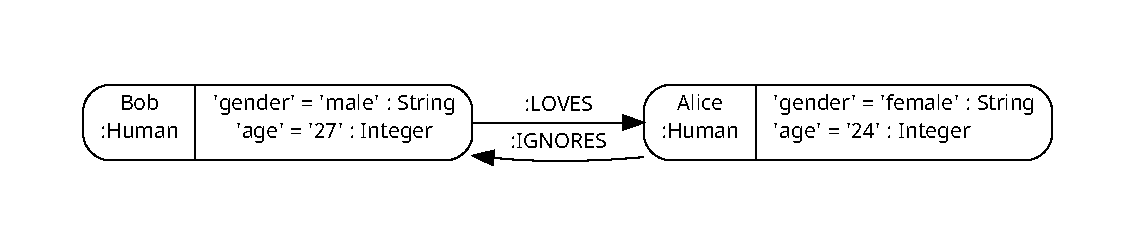
\includegraphics[width=\textwidth, trim=12mm 12mm 12mm 12mm,clip]{figures/property-graph.pdf}
    \caption{Two persons' relationship modeled with a property graph}
    \label{fig:property-graph}
\end{figure}

\subsection{Neo4j}
\label{subsection:preliminaryneo4j}

Among a handful of graph database vendors~\cite{graph-dbs}, Neo Technology's Neo4j is the most popular one~\cite{graph-dbs-raking}. It features full ACID-compliance upon a pure graph data model, contrary to other vendors' multi-model approaches. Besides Neo Technology, Neo4j is backed by the open-source community as well~\cite{neo4j-github}. There are two variants: \emph{Community Edition} and \emph{Enterprise Edition} with an extended feature set~\cite{neo4j-licensing}. Neo4j also offers a program tailored to startup companies~\cite{neo4j-startup-program}. With the help of this startup program, companies can build their applications on the Enterprise Edition of the Neo4j platform, free of charge.\footnote{Certain limitations apply: the company must have at most 50 employees and at most \$3 million annual revenue, among others~\cite{neo4j-startup-program}.}

\subsection{Cypher}

Cypher is a query language developed especially for graph databases by Neo Technology~\cite{neo4j-cypher}. \Cref{fig:cypher-intro} shows that the language uses a sort of ASCII-art to represent nodes and relationships: nodes are in parentheses, relationships are in brackets surrounded by relationship direction information.

\begin{figure}[!htb]
    \centering
    \lstinline{(Bob)-[:LOVES]->(Alice)}
    \caption{A basic Cypher example}
    \label{fig:cypher-intro}
\end{figure}

Cypher syntax is elegant and expressive, thus very readable. Besides using it to represent nodes and relationships, we can utilize it to access the Neo4j's indexing capabilities and stored procedures as well. Even complex pattern-matching conditions can be expressed easily and intuitively in Cypher. Although today's modern application development frameworks — adopting increasingly capable data mapping solutions — make it less and less necessary to directly interact with databases, complex queries can still involve composing database commands manually. Therefore the expressiveness and ease of use of a database query language still remains essential.

\section{Git and GitHub}

I have been maintaining altogether 9 projects related to Diplomatiq, all being tracked by a version control system, Git. I chose Git because of its maturity\footnote{Git has been developed since 2005~\cite{git-initial-commit}.} and popularity, and also because of the fact that this is the versioning tool that I am most experienced with. For open-source software maintenance, I chose GitHub, as it is the most popular software collaboration platform~\footnote{GitHub has over 40 million users~\cite{github-user-count}.}, and offers advanced development and project management tools, security settings, and a full-featured, integrated testing infrastructure. Also, it enables to maintain repositories under a larger unit, called organization, offering sophisticated administrative and security features. GitHub is free of charge for open-source projects~\cite{github-pricing}.

\section{Microsoft Azure}

Having relevant work experience in operating a production cloud server infrastructure, I had a concrete concept on Diplomatiq's demands on the short and on the run as well. The key aspects of choosing the platform were the following:

\begin{itemize}
\item It should provide strong cloud-based services with hybrid cloud\footnote{A hybrid cloud consists of cloud-based and on-premise infrastructure elements.} capabilities for later expansion into real-world diplomacy.\footnote{According to my knowledge, governmental and diplomatic software often require on-premise solutions.}
\item It should provide strong PaaS\footnote{Platform-as-a-Service} capabilities, and also IaaS\footnote{Infrastructure-as-a-Service} solutions.
\item It should provide options on data residency to comply with diplomatic requirements.
\item It should offer a flexible pricing model, so I can start with a smaller, cheaper infrastructure, and scale it later as Diplomatiq's production workload grows.
\item It should provide mature, integrated security solutions.
\item It should provide affordable developer support.
\end{itemize}

Considering the above, I evaluated service offerings of Microsoft Azure, Google Cloud Platform, and Amazon Web Services. Google seems to lag behind on hybrid solutions, and also seems to be the worst from the financial aspect for Diplomatiq's use cases. Even though Amazon is the oldest cloud service, it seems to lack integrated data residency solutions. Microsoft seems to offer everything Diplomatiq will need in the long run, and it proved to be the best in terms of pricing, therefore I chose Microsoft Azure as Diplomatiq's cloud server infrastructure platform.

\chapter{Building and securing a company-level production infrastructure}
\label{chapter:infrastructure}

This chapter describes my approach of building and securing a production-grade infrastructure supporting the development, testing, and public operation of Diplomatiq.

\section{Introduction}

The underlying infrastructure plays a foundational role in the eventual success or failure of every business. 21\textsuperscript{st}-century companies often build their business operations entirely on information technology solutions, meaning a well-founded IT infrastructure is key to succeed. Even though at the time of writing this thesis, Diplomatiq is a company existing only in the future, the infrastructure I elaborate in the present will be the foundation of its business operation. By setting up a robust and secure infrastructure, I want to establish the future of Diplomatiq. It needs to be done right, so it does not need to be done again.

This involves two principles. The first is that key infrastructure elements need to be established using mature and robust solutions, so they do not need to be rebuilt or replaced later. This excludes trial versions of services, expiring student offers, and generally free solutions as well. Organizational hierarchy needs to be set up properly, allowing later expansion, and the infrastructure with all its access credentials should be documented meticulously. The second principle is that security should be taken into consideration from the very beginning. Authentication and authorization policies should be the as strict as possible, and all access credentials should be stored in a safely encrypted manner.

Throughout this chapter, I introduce the various infrastructure elements I evaluated, purchased and integrated into Diplomatiq's infrastructure. Security-related aspects will appear in most of the sections.

\section{Naming}
\label{section:naming}

A good brand name identifies a company in various ways. Apart from marketing purposes, the name should be suifficently unique to be usable within the various services and namespaces on the Internet. For this purpose, \emph{Diplomatiq} seemed to be suitable: it is unique, appropriately short for both domain names~\cite{howtochoosedomainname} and the human memory~\cite{memoryfour} with its 10~characters, and it characterizes its subject well.

I formulated the following — prioritized — guidelines for reserving namespaces for Diplomatiq across services on the Internet:

\begin{enumerate}
\item If available, use \emph{Diplomatiq} (capitalized).
\item Else if the service allows lowercase letters only, use \emph{diplomatiq}.
\item Else if use \emph{DiplomatiqOrg} (capitalized).
\item Else if use \emph{diplomatiqorg}.
\item Else use a custom name.
\end{enumerate}

As of now, there has been no need to apply the 5\textsuperscript{th} rule.

\section{Brand}

For visual recognition, a company needs a well-defined image. Diplomatiq's corporate identity was designed by one of my acquaintances, Roland Hidvégi. It includes a logotype, three variants of application icons, ten brand colors, and Eina~\cite{eina} as the advised font family\footnote{As Eina is not available as a free web font~\cite{eina-licensing}, I temporarily use Helvetica instead.}. \Cref{fig:diplomatiq-logotype} and \Cref{fig:diplomatiq-app-icons} shows the logotype and the application icon variants.

\begin{figure}[!htb]
    \centering
    \vspace{2mm}
    
\includegraphics[width=8cm]{figures/diplomatiq-logo.pdf}
    \caption{The logotype of Diplomatiq}
    \label{fig:diplomatiq-logotype}
\end{figure}

\begin{figure}[!htb]
    \centering
    
\includegraphics[width=8cm]{figures/diplomatiq-app-icons.pdf}
    \caption{The application icon variants of Diplomatiq}
    \label{fig:diplomatiq-app-icons}
\end{figure}

\section{Domain name}

\subsection{Overview and purchasing the domain name}

A domain name in the Domain Name System (DNS) represents a network domain, or it translates to an Internet Protocol address~\cite{rfc1035}. Having a domain name is necessary for companies with web-facing services, both for users to easily memorize the address of the service, and for deploying security measures, such as Transport Layer Security (TLS)~\cite{rfc8446}. As Diplomatiq is not primarily a commercial entity, but rather a diplomatic organization, I decided its domain name to be \lstinline{diplomatiq.org}. Since I was already registered at the domain name registrar Namecheap~\cite{namecheap-website}, it was starightforward to purchase the domain name from them, under my existing user account. I set up various DNS records for deployed services, these will be detailed later at describing the services themselves.

\subsection{Security}

Even though I have a secure, long, cryptographically random password for my Namecheap account — as well as for every other user account I have — and I store it in an encrypted password manager, I enabled multi-factor authentication, to reduce the possibility of an unauthorized party accessing Diplomatiq's DNS infrastructure. I also turned on all security alerts to get immediately notified about all events regarding the domain.

I deployed DNS Security Extensions (DNSSEC) under the Diplomatiq domain. DNSSEC essentially prevents spoofing DNS data by providing a set of methods to DNS clients to cryptographically authenticate the integrity and existence (or non-existence) of DNS records~\cite{rfc4033}. Although there is a long-standing debate about the usefulness and operational security of DNSSEC~\cite{4159821, ptacek-dnssec-rant-2, ptacek-dnssec-rant-1}, I decided that until it does not cause any failures or outages in production, it will be enabled.

\section{TLS infrastructure}

\subsection{Overview}

Transport Layer Security (TLS) is a cryptographic protocol with the goal of providing a secure channel between two communicating parties — usually between a client and a server — over the Internet, offering cryptographic assurances for the following:

\begin{itemize}
\item \emph{Authentication} with public-key (asymmetric) cryptography. In TLS, the server is always authenticated, and the client is optionally authenticated.
\item \emph{Confidentiality} with secret-key (symmetric) cryptography. Data sent over the channel is encrypted in transit.
\item \emph{Integrity} with cryptographic message-authentication codes. Data sent over the channel cannot be modified without detection~\cite{rfc8446}.
\end{itemize}

For protecting web application users and web API\footnote{Application Programming Interfaces define interactions between softwares. In this context, a web API means a web-facing service, which serves data for client applications.} consumers on the Internet, a web server should serve its contents over TLS, e.g.\ over the HTTPS protocol, which is essentially HTTP over TLS. More and more web browser APIs require websites and web applications to be served over HTTPS~\cite{secure-context-features}.

Authenticating the server involves a digital certificate, which proves the ownership of the server's \emph{public key}. The public key and its cryptographic key pair, the \emph{private key} are involved in the cryptographic key handshake of TLS, resulting in a symmetric key for encrypting data in transit. Certificates are issued to one or more specific domain names, cryptographically signed by a trusted third party called a Certificate Authority (CA)\footnote{For the sake of compactness, I will not go into the endless details of the X.509 certificate infrastructure and the underlying public-key cryptography in this thesis.}. Acquiring such a certificate requires proving the ownership of the domain names in question. \emph{Non-wildcard certificates} only certify domain names they were issued to, whereas \emph{wildcard certificates} certify given domains and all their immediate subdomains.

\subsection{Purchasing a TLS certificate}

Having a TLS certificate signed by a trusted CA is a requirement of serving content over HTTPS, thus it is necessary — but not sufficient on its own — for securing web applications and web APIs. Such certificates can be purchased from a multitude of vendors. For \lstinline{diplomatiq.org}, I purchased a TLS certificate from Sectigo, one of the leading TLS certificate vendors in the world~\cite{sectigo-website}. The certificate is issued to the domain names \lstinline{diplomatiq.org} and \lstinline{www.diplomatiq.org}, and since it is a non-wildcard certificate, I will need to acquire additional certificates for other subdomains.

\subsection{Security}

The private key of a certificate is a highly sensitive secret. An attacker obtaining the private key of a server certificate is able to decrypt all trafic sent to and received by the server, or it can even modify the data in transit, tricking the user into surrendering sensitive information, such as passwords. While being stored securely, the private key needs to be always available to the server, as it is constantly involved in the communication.

The private key of the certificate issued to \lstinline{diplomatiq.org} is encrypted with a long, cryptographically random password, and it is stored in a cryptographic Hardware Security Module\footnote{Hardware Security Modules are separate physical computers designed to keep cryptographic keys safe. They offer tamper resistance making it extremely difficult to extract and steal secret keys~\cite{fips-140-3}.} by Microsoft Azure's Key Vault\footnote{Microsoft Azure and its Key Vault service in particular will be detailed later.} service. This way, the private key is only available in an audited, secure manner, guarded by strict access policies.

As an additional safety measure, I deployed \emph{Certification Authority Authorization (CAA)} DNS records for \lstinline{diplomatiq.org}. CAA records specify authorized CAs, which are allowed to issue certificates for the given domains~\cite{rfc8659}. The records essentially form a CA whitelist, preventing the mis-issue of valid TLS certificates by unauthorized parties. I set up CAA records as granularly as possible: every subdomain has its own authorization. I specified Sectigo for the apex domain \lstinline{diplomatiq.org} and the subdomain \lstinline{www.diplomatiq.org}, DigiCert for the subdomains \lstinline{app.diplomatiq.org} and \lstinline{api.diplomatiq.org}, and Let's Encrypt for the subdomain \lstinline{neo4j.diplomatiq.org}. DNSSEC prevents spoofing additional CAA records into the Diplomatiq domain.

Diplomatiq currently only makes use of server certificates for supporting TLS on its website, web application and web API. Possible future uses of certificates include signing released software with a code signing certificate, or authenticating API clients with client certificates.

\section{Email infrastructure}

\subsection{Overview and usages}

The ability of sending and receiving emails is a basic business requirement for communicating with business clients and service providers. In the following, I will refer these as \emph{individual emails}, as they are mostly initiated by a human individual. Also, application development often demands sending automated \emph{transactional emails} for customers, as well as \emph{promotional emails} delivering marketing campaigns and promotions.

\subsection{Sending and receiving individual emails}

Namecheap offers basic email forwarding capabilities along with its DNS service I subscribed to. Even though certain business email providers offer more robust — and also more expensive — solutions, I decided that my current requirements are covered by forwarding emails received by any address ending with \lstinline{@diplomatiq.org} to my personal email address. I also managed to configure my personal email provider to send emails in the name of several \lstinline{@diplomatiq.org} email addresses through SendGrid, a service for delivering transactional and promotional emails~\cite{sendgrid-website}. For achieving this, I needed to set up separate email entities in my personal email provider to send emails through SendGrid's SMTP-over-TLS API, authenticated by a newly created API key.

Currently several email addresses are configured with the above method, each used for different purposes in different services. Dedicated \emph{per-service email addresses} are useful for services lacking federated authentication and role-based access control features, as they enable to distribute reponsibilities among colleagues by providing access to the email addresses, without irrevocably binding those responsibilities to the colleagues' email addresses. The configured email addresses with their usage are available in the Appendix.

\subsection{Transactional and marketing emails}

For delivering transactional and marketing emails, I subscribed to SendGrid's smallest paid plan, which includes 40,000 sent emails per month. The service allows to create rich-text email templates in its online editor, then send personalized emails to multiple addresses, by substituting template placeholders with per-user customized data. I configured SendGrid to use the \lstinline{team@diplomatiq.org} email address for all outgoing email communication. Configuring the service to access and use the \lstinline{diplomatiq.org} domain was straightforward: it only involved adding generated \lstinline{CNAME} records to the DNS configuration.

\subsection{Securing SendGrid access}

Since SendGrid offers neither federated nor email-based user management, I created a new account with a username. I enabled two-factor authentication for the service, and I defined various alerts for account access and quota usage. I also introduced IP address-based access controls: my user account is accessible only from my static home IP address and my private VPN\footnote{Virtual Private Network}\footnote{I have a personal VPN hosted by a self-configured virtual machine in a data center. The VPN's IP address is also allowed to access SendGrid, so I can log in to my account even if I am not home.}, and the SendGrid API authenticated by my API keys is only accessible from the IP range of the production server infrastructure, which I will detail later. The issued API keys have minimal privileges allowing email sending only.

\subsection{Securing emails sent by Diplomatiq}

Sending emails over the Internet is inherently insecure, as the design of the core email protocols do not incorporate any security features for sender authentication and authorization~\cite{foster2015security}. The infrastructure on its own allows anyone to send emails from any domain, without verifying the authenticity of the sender~\cite{rfc5321}. There are several additional security measures to mitigate this threat, such as the Sender Policy Framework~\cite{rfc7208}, DomainKeys Identified Mail Signatures~\cite{rfc6376}, and the Domain-based Message Authentication, Reporting, and Conformance~\cite{rfc7489} protocols. I have applied all three of them for Diplomatiq.

The Sender Policy Framework (SPF) was designed to detect if the sender address of an email was forged by a party outside the sender's domain. The framework's operation is based on a DNS TXT record\footnote{The SPF record has a specific format, which is defined in RFC 7208~\cite{rfc7208}.} indicating the host or IP address of email servers authorized to send emails originating from the domain. Besides authorized servers, the record also includes instructions for recipient servers and clients on what to do with detected forgeries: such emails can either be forwarded to the recipient's mailbox tagged as spam, or rejected and not delivered. Diplomatiq's SPF policy is configured by Namecheap and SendGrid based on my settings, and it commands to reject emails detected as forgeries.

The DomainKeys Identified Mail (DKIM) Signatures scheme offers similar email sender forgery detection capabilities as the Sender Policy Framework, but also it provides additional assurances supported by public-key cryptography. For utilizing DKIM, the sender server needs to cryptographically sign outgoing emails with a private key, and the domain's administrators need to publish the server's corresponding public key in a DNS TXT record\footnote{The DKIM record contains additional information besides the key itself. The format of the record is specified by RFC 6376~\cite{rfc6376}.}. Recipient email servers and clients can check the authenticity of an email by looking up the sender domain's public DKIM key then verifying the DKIM signature attached to the email\footnote{DKIM signatures are usually verified by email clients rather than end-users, thus the signatures are generally not visible as part of the email.} with the public key. On the one hand, a valid DKIM signature cryptographically guarantees that the email was sent from an authorized party, and on the other hand, it also verifies that the email was not modified in transit. I configured the DKIM records of Diplomatiq to be automatically managed by Namecheap and SendGrid.

The Domain-based Message Authentication, Reporting and Conformance (DMARC) protocol extends SPF and DKIM by allowing domain administrators to explicitly indicate that emails are to be authenticated by SPF or DKIM or both, and to instruct email recipient clients to behave in a specific way when any or all authentications fail, such as rejecting the message, or putting it in quarantine. DMARC also offers a reporting mechanism, which sends reports about authentication failures to a specified email address. Reports can be daily aggregates or real-time \textquote{forensic} reports including detailed data about each failures, or both. Diplomatiq's DMARC policy is set to the strictest: emails not passing all checks should not be delivered to the recipient's inbox. For receiving and analyzing aggregate reports, I use an external tool, called Dmarcian~\cite{dmarcian-website}. DNSSEC prevents the unauthorized modification of Diplomatiq's SPF, DKIM and DMARC policies.

\section{Source code management}

\subsection{Choosing tools}

I have been maintaining altogether 9 projects related to Diplomatiq, all being tracked by a version control system, Git. I chose Git because of its maturity\footnote{Git has been developed since 2005~\cite{git-initial-commit}.} and popularity, and also because of the fact that this is the versioning tool that I am most experienced with. For open-source software maintenance, I chose GitHub, as it is the most popular software collaboration platform~\footnote{GitHub has over 40 million users~\cite{github-user-count}.}, and offers advanced development and project management tools, security settings, and a full-featured, integrated testing infrastructure. Also, it enables to maintain repositories under a larger unit, called organization, offering sophisticated administrative and security features. GitHub is free of charge for open-source projects~\cite{github-pricing}.

\subsection{Registering the Diplomatiq GitHub organization}

I registered an organization on GitHub under the name \emph{Diplomatiq}. I uploaded all necessary data including logos, descriptions, general and billing email addresses, and website addresses. Considering future employees, I made it mandatory for all members of the organization to use two-factor authentication. I verified my ownership of the \lstinline{diplomatiq.org} domain to GitHub with a custom DNS TXT record, thus GitHub displays a \textquote{Verified} label next to Diplomatiq's website address. For making future collaborative development eaiser, I added a set of organization-wide issue and pull request labels, making sure all repositories I create have the same issue types.

\subsection{Standardized, organization-wide documents and configurations}

As I created more projects, I experienced that certain documents, templates and configurations need to be present in all of projects, mainly because of the recommended open-source community standards maintained by GitHub~\cite{opensource-guide}. For being able to instantly create a new project with Diplomatiq's standardized project structure containing all such necessary files, I created another project called \emph{project-config}, which will be described in \Cref{chapter:libraries}.

\subsubsection{License}

The most basic project requirement is a license. Within Diplomatiq, project licenses are stored in a file called \lstinline{LICENSE} within the project's root directory. This is in line with GitHub's recommendations, thus the platform can automatically parse and display license information. Currently all Diplomatiq projects are licensed under the MIT License~\cite{mit-license}.

\subsubsection{Readme}

All projects are initialized with a \lstinline{README.md} file containing the project's name and description. I put all project documentation into the readme file for most projects, thus these files are not left empty. I usually also include badges into readme files about build status, versioning and license information, as well as code quality and code coverage data.

\subsubsection{Code of conduct}

Code of conduct documents formulate a set of ethical norms and responsibilities on practices of collaboration. Diplomatiq uses the version 1.4 of the Contributor Convenant's Code of Conduct across all its projects, in a file named \lstinline{CODE_OF_CONDUCT.md}. Even though currently there is no open-source collaboration in Diplomatiq's repositories, once we get there, I want to take the Code of Conduct very seriously, in order to create a welcoming and inclusive development environment. I have already configured the \emph{conduct@diplomatiq.org} email address for reporting unacceptable behaviour.

\subsubsection{Contributing information}

The document \lstinline{CONTRIBUTING.md} — named in line with GitHub's open source recommendations — summarizes how to contribute to Diplomatiq projects. It describes means of communication with project maintainers, and methods of requesting features and reporting bugs. It formulates a set of submission guidelines for issues and pull requests. It also presents a style guide for the code itself, and for commit messages. As I adopted the Angular-style Conventional Commits specification~\cite{conventionalcommits}, the document introduces the concept conventional commit messages in an example-based manner.

\subsubsection{Pull request template}

In order to discourage future contributors from submitting incomplete work, I prepared a checklist as part of GitHub's pull request template. As the checklist is saved into the file called \lstinline{.github/PULL_REQUEST_TEMPLATE.md}, GitHub displays it as the initial contents of the to-be-submitted pull request's details field. The checklist requires:

\begin{itemize}
\item the pull request to consist of one commit;
\item the commit message to follow the commit message guidelines;
\item the tests to be updated (if applicable);
\item the documentation to be updated (if applicable).
\end{itemize}

Beyond the checklist, the template instructs the developer to indicate the pull request's type, describe the application behavior the pull request modifies, describe the new behaviour, and indicate if the pull request introduces a breaking change.

\subsubsection{Issue templates}

In open-source projects, it is common that developers submit issues without describing clear and concise details. To discourage this routine, I created two types of issue templates. When developers want to create a new issue in a repository, they are offered these issue templates to choose from. The \emph{bug report} template encourage developers to detail the perceived failure as much as possible, and to disclose the execution context, expected behaviour and steps of reproduction. The \emph{feature request} template supports the issuer in describing their exact requirements along with considered solutions, if there are any.

\subsubsection{.editorconfig file}

EditorConfig helps maintain consistent coding styles for multiple developers working on the same project across various editors and IDEs. The EditorConfig project consists of a file format for defining coding styles and a collection of text editor plugins that enable editors to read the file format and adhere to defined styles~\cite{editorconfig}.

\subsubsection{Security policy}

Since exploiting security vulnerabilities can lead to catastrophic consequences like data breaches or loss of data, security issues are to be handled carefully and discreetly. A security policy establishes rules and methods for reporting a security issue in a development project to the maintainers without causing any harm. Diplomatiq's security policy requires contributors to report found security issues to the \emph{security@diplomatiq.org} email address, possibly encrypted with Diplomatiq's public PGP key\footnote{Diplomatiq's public PGP key is available on the https://www.diplomatiq.org/pgp-key.txt URL.}.

\subsection{Development and release model}

In most of Diplomatiq's repositories, I use the a modified version of the GitFlow workflow~\cite{gitflow}. In essence, the workflow operates on four types of branches in a repository:

\begin{enumerate}
\item The \emph{master} branch is stable, and should be kept stable at all times. Code gets merged into the master branch only from a \emph{release} branch, immediately before a new version of the software is released into production\footnote{As described later, most Diplomatiq projects are configured in a way that merging a tagged commit into the master branch triggers the continuous delivery flow and deploys the version into production.}. Contributors can not push code directly onto this branch, but administrators can.
\item The \emph{develop} branch is part of the repository's regular development flow. When creating feature branches, contributors branch from develop, and the target of contributional pull requests is the develop branch. Contributors can not push code directly onto this branch, but administrators can.
\item The \emph{feature/*} branches are also parts of the regular development flow. Contributors develop their contributions on feature branches, regardless of the contribution's type (feature, bugfix, refactor, etc.). Contributional pull requests are created from feature branches targeting develop.
\item The \emph{release/*} branches are created when a release candidate is being prepared, by branching from develop. Release-related code changes like version bumps, changelog generation and release hotfixes are committed onto the release candidate's release branch, and eventually the finalized release candidate is tagged. After conducting all necessary testing on the release candidate, the release branch is merged into master, then it is immediately released into production by continuous delivery. After the deployment finished, the release branch is merged into develop. Contributors can not push code directly onto release branches, but administrators can.
\end{enumerate}

\Cref{fig:git-workflow} displays the above workflow, which can be well supported by GitHub's continuous integration and continuous delivery capabilities and branch protection rules. I created such rules for the \emph{master}, \emph{develop}, and \emph{release/*} branches. All branches require certain status checks to pass before merging code into the mentioned branches, and require the merged branches to be up to date when merging. As a general rule, I also require linear history in Diplomatiq's repositories, because I experienced that this way tasks such as automated changelog generation or finding regressions with \lstinline{git bisect} becomes easier.

\begin{figure}[!htb]
    \centering
    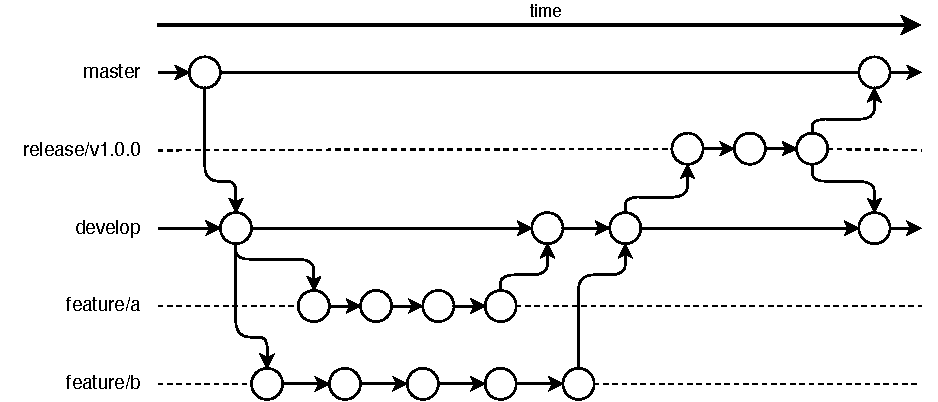
\includegraphics[width=\textwidth]{figures/git-workflow.pdf}
    \caption{Diplomatiq's modified version of the GitFlow workflow}
    \label{fig:git-workflow}
\end{figure}

I implemented a versioning strategy following the scheme of semantic versioning. This scheme defines the software version as a numeric triplet separated by dots in the form \lstinline{MAJOR.MINOR.PATCH}. The \lstinline{MAJOR} version is to be incremented in case the version contains incompatible API changes, the \lstinline{MINOR} version is to be incremented if the version's added functionality is backwards compatible, and the \lstinline{PATCH} version is to be incremented if the version solely consists of backwards compatible bug fixes~\cite{semver}. Adhering to the above helps managing software versions and dependencies with a lesser chance to introduce unintended breaking changes.

As Diplomatiq's development and release model features both conventional commits and semantic versioning, it was straightforward to implement automated changelog generation as well. Using Conventional Changelog Tools~\cite{conventional-changelog}, I automatically generate each released version's changelog from the commit messages contained by the version.

\subsection{Automated dependency management}

As development and release processes become more and more automated, the time frame required for releasing new software versions reduces. With continuous delivery, pushing new code into the remote repository often means that the code is released to production without further developer interaction, after all necessary automated tests pass. This results in the need of more frequent dependency updates as well. Maintainers can either check and update every dependency manually, or they can apply automated solutions.

I have configured Dependabot for the automatic maintenance of dependencies across Diplomatiq projects. Dependabot is a GitHub-owned, integrated tool for watching package managers like NPM and Maven, continuously checking for new versions published. I set up Dependabot in a way that if it detects one of the dependencies in Diplomatiq projects having a new version released, it opens a pull request in the related project with the dependency update. This automated workflow frees me from a lot of manual work, and also ensures that the dependencies of Diplomatiq projects are always up to date. Pull requests containing security-related updates are separately tagged, allowing me to handle them with higher priority. As I do not want to lose the ability of reviewing dependency updates, merging pull requests opened by Dependabot is not automated. But since continuous integration workflows are applied to all pull requests, all checks and tests defined in the repository are run for Dependabot's updates as well as for any other contribution.

\subsection{Continuous integration and continuous delivery}

Martin Fowler defines continuous integration (CI) as a software development practice where team members integrate their code changes into the repository mainline frequently, at least daily, and each integrations are verified by a set of automated build and test methods in order to detect integration errors as soon as possible. According to Fowler, this leads to less integration problems, and faster development and release cycles~\cite{fowler-ci}.

In case of Diplomatiq projects, the repository mainline is the develop branch, and the integrations are essentially pull requests opened by repository contributors. The set of automated build and test methods applied to pull requests vary across projects according to the chosen technology, language, and framework, but Diplomatiq libraries and production software usually contain automated tests for verifying conformance, functional correctness, and adherence to various code quality metrics.

I configured all projects to use GitHub Actions~\cite{githubactions} for continuous integration (and continuous delivery). Previously I used the mature and well-supported Travis CI~\cite{travisci}, but encountering constant stability problems with Travis made me to switch to the then freshly announced GitHub Actions. Since the switch, I experienced GitHub Actions to be a well-founded, stable solution. As it is an integral part of the GitHub platform, it furthers the possibilities of integrations by allowing to subscribe to more repository events than external platforms~\cite{actions-events}. It also enables to utilize GitHub's REST and GraphQL APIs for extending the base functionality of GitHub Actions with built-in authentication — a feature I make use of in almost all projects.

GitHub Actions essentially allows to create custom, automated \emph{workflows} for various phases of the software development lifecycle. Such workflows are declaratively defined in a YAML\footnote{Yet Another Markup Language is a markup language for human-readable configuration and serialization.} files, stored in the repository alongside the project's sourcecode. Workflows are triggered by GitHub's \emph{events}, and consist of \emph{jobs} able to run sequentially on different {runners} having different operating systems. Jobs encompass \emph{steps}, the smallest work unit within a workflow. Steps are either predefined \emph{actions} stored in public repositories and created by GitHub members, or shell scripts.

Although different projects require different CI workflows, I have established the following baseline for checking contributions across Diplomatiq projects:

\begin{itemize}
\item If the workflow was triggered by a pull request, check if the pull request consists of one commit. This involves substeps of querying the number of commits for the pull request through GitHub's GraphQL API, extracting the number of commits from the JSON response, and checking if the number is equal to 1.
\item Check if the commit message conforms to the requirements of Angular-style conventional commits. The commit message is linted with the \emph{commitlint} tool, part of the previously mentioned Conventional Changelog Tools.
\item After setting up the project's programming language environment and installing all necessary dependencies, perform code linting in order to verify that the submitted code conforms to the required code styling of Diplomatiq. The code is linted with language-dependant tools.
\item Verify that the project can be built by creating a distribution deployment artefact.
\item Run all unit, integration, and end-to-end tests of the project, if there are any.
\item Scan the code with SonarQube, and upload the results to SonarCloud.
\end{itemize}

If any of the above steps fails, the contrubition should be considered as faulty, and it should not be accepted into the mainline. Since all Diplomatiq projects are open-source, and GitHub Actions is offered free of charge for open-source projects, I usually run workflows incorporating the above steps against multiple platforms, operating systems, and multiple versions of programming language environments concurrently, without additional costs.

I also utilize GitHub Actions for continuous delivery. Most projects are configured in a way that pushing a tagged commit to the master branch triggers the release process. The process consists of producing and uploading a distribution build artefact to GitHub's permanent artefact storage, running all tests against all environments on the artefact, and if everything step is successful, deploying the artefact into the production infrastructure.

\subsection{Code analysis with SonarCloud}

SonarSource's SonarQube along with its cloud platform, SonarCloud are tools for inspecting code quality based on static code analysis. Both examine the code using the same configurable — and in case of SonarQube, extensible — analysis ruleset in order to detect bugs and security vulnerabilities. SonarQube is to be used in on-premise, SonarCloud is to be used in cloud-based development environments, and both can be included in continuous integration environments.

As it is free to use for open-source development, I configured SonarCloud for most Diplomatiq projects. After creating the Diplomatiq organization on the platform, I imported the Diplomatiq's GitHub repositories into SonarCloud through an automated flow. I created a token for each project, which authenticates the project against SonarCloud's API when performing analyses and uploading results.

SonarCloud introduces the concepts of \emph{quality profiles} and \emph{quality gates}. A quality profile is a set of language-dependant quality rules, which get applied against the codebase during an analysis. Profiles are categorized into four parts:

\begin{enumerate}
\item \emph{Bugs} are development errors which occasionally result in faulty software.
\item \emph{Vulnerabilities} are pieces of code that causes the software to become vulnerable against attacks.
\item \emph{Code smells} are bad coding practices which make the code harder to maintain.
\item \emph{Security hotspots} are subject to become vulnerabilities if applied incorrectly.
\end{enumerate}

An example of a quality rule categorized as a bug in the Java quality profile is the reversion of the \textquote{not equals} operator (incorrectly using \lstinline{=!} instead of the correct \lstinline{!=}): the code compiles, but the operator does not produce the intended results. Quality profiles can be customized by including or excluding specific rules. When using SonarQube, new quality rules can also be implemented for several languages, but SonarCloud can not be extended with custom rules~\cite{sonar-custom-rules}. For Diplomatiq projects, I use the quality profiles recommended and maintained by SonarSource.

A quality gate is a set of boolean conditions based on measurement values. Such conditions are not dependent on any language or platforms, since it formulates general measurements, such as code coverage should be kept above a specific percentage, the number of bugs should be equal to zero, or security rating should be the highest. A quality gate \textquote{lets through} code which complies with all its requirements. For Diplomatiq projects, I use a custom quality gate with the highest and strictest possible settings on the platform.

As I configured SonarCloud to be part of the continuous integration workflows of Diplomatiq projects, only such pull requests can be merged into a Diplomatiq repository, which passes all requirements I set in SonarCloud. Since the CI rules of GitHub projects apply to me as well as any other future contributor, this enforces even me to write code with consistently high quality and 100\% test coverage\footnote{I always strive to produce high quality code and avoid bugs. However, SonarCloud helped me to notice two minor bugs so far, which were not reported by tests, not even with the 100\% test coverage.}.

\section{Node Package Manager (NPM)}

\subsection{Overview}

The Node Package Manager (NPM) — part of an ecosystem built upon the JavaScript runtime environment Node.js — is a package manager for software written in JavaScript. NPM's online package registry containing public and private packages enables developers to download and re-use shared packages by incorporating them into their own software in a versioned manner, with the help of NPM's command line client. It has become the de-facto standard solution for sharing JavaScript software in the open-source community~\cite{herron2016node}.

\subsection{Creating and securing an organization}

I implemented several JavaScript libraries to be published as open-source software, but in Diplomatiq's name instead of my personal account. For this, I created an organization on NPM, similarly to GitHub. Organizations can publish packages in a scoped way: the name of the organization prefixed with a \textquote{@} character — the scope name — becomes the prefix of the package's name. The scope and the package name are separated with a \textquote{/} character. For example, the \lstinline{project-config} package published under the Diplomatiq organization gets finally named \lstinline{@diplomatiq/project-config}\footnote{NPM scopes can be lowercase only, so according to Diplomatiq's naming rules described in \Cref{section:naming}, the organization's scope has been \lstinline{@diplomatiq}.}.

NPM offers no security policies for organizations. As a security measure, all I was able to do was to enable two-factor authentication in my account for publishing packages as well, as it was of course already enabled for authentication. This means that if I invite a user into Diplomatiq's NPM organization, they will be able to publish packages even if they do not have two-factor authentication enabled. This way, an attacker stealing the password of one of the organization's future accounts can easily compromise Diplomatiq packages. I contacted NPM's customer support about mitigating this future threat, and I was told that the functionality of organizational policies are on their development roadmap, expected to be released to production in the fourth quarter of 2020.

\section{Communication and social media presence}

\subsection{Gitter}

I created a space for Diplomatiq on Gitter, a chat service for GitHub repositories and developers. The space was named Diplomatiq, according to the primary naming rule in \Cref{section:naming}. Gitter allows to create several chat rooms within Diplomatiq's space, corresponding to the repositories within Diplomatiq's GitHub organization. As advised in Diplomatiq's contributing guide, the Gitter space should be the primary place for discussing questions and problems regarding Diplomatiq projects. At the time of writing this thesis, I am the sole member of Diplomatiq's Gitter space, and there has been no communication in the chat rooms.

\subsection{Slack}

For future internal communication, I registered a workspace for Diplomatiq on Slack, one of today's most popular business communication platforms. The workspace was named Diplomatiq, but due to the \emph{diplomatiq.slack.com} domain being already taken, its domain name has been \emph{diplomatiqorg.slack.com}, according to the 4\textsuperscript{th} naming rule in \Cref{section:naming}. Even though the workspace is unused as I am its sole member, reserving \emph{diplomatiqorg.slack.com} ensures that the domain name will not be taken by another company. As a security measure, I made it mandatory for all future members to use two-factor authentication.

\subsection{Facebook}

I created and published a Facebook page for Diplomatiq, reserving the Facebook page path \emph{https://www.facebook.com/DiplomatiqOrg}, according to the 3\textsuperscript{rd} naming rule of \Cref{section:naming}. The page has no posts and contains no data, but I uploaded one of Diplomatiq's application icon as its profile picture, and the logo as its cover picture. In the future, I want to heavily build on Diplomatiq's Facebook presence for reaching the younger generation of Model United Nations.

\section{Procuring the Neo4j database software}

\subsection{Licensing overview}

I chose the Neo4j graph database as the main database serving the Diplomatiq social network application. The reasons of my decision are detailed in \Cref{section:database}, this section focuses on licensing and the procurement of the database software.

As already mentioned in \Cref{subsection:preliminaryneo4j}, Neo4j offers two software editions with different feature sets and licensing~\cite{neo4j-licensing}. The Community Edition is open source, available under the terms of the GPL v3 license. The Enterprise Edition offers four licensing options:

\begin{itemize}
\item The commercial license permits using the software in closed source applications as well, and is offered under a paid subscription agreement.
\item The developer license permits free local development usage after registration.
\item The evaluation license is a time-restricted variant of the commercial license, offering free usage for a fixed-term trial period.
\item The startup license permits using the software for free for startups having at most 50 employees and \$3 million of annual revenue, but limits the number of database instances to 3 production, 3 staging, and 6 testing/development machines, each having 256 gigabytes of RAM and 24 processor cores at most~\cite{neo4j-startup-program}.
\end{itemize}

Besides the software itself, Neo Technology offers another approach for using their graph database: Neo4j Aura is a managed graph DBaaS\footnote{database as a service}, offering on-demand scaling, a capacity-based pricing construction, and clustering features for high availability.

\subsection{Acquiring the startup license}

After evaluating licensing options and the Neo4j Aura service, I decided that since Aura is too expensive for my current budget, I enroll in the startup program. This involved filling a registration form with personal data and information about the (prospective) company. Two days after submitting the form, I received the email with a license key for Neo4j Enterprise Edition. This enabled me to download and deploy the software onto Diplomatiq's server infrastructure.

\section{Building and securing the server infrastructure}

\subsection{Platform overview}

In this section, I use the term server infrastructure to denote the various servers, software, networking solutions, and configurations that enables and supports the public operation of the Diplomatiq social network software system on the Internet (excluding DNS and emailing). Having relevant work experience in operating a production cloud server infrastructure, I had a concrete concept on Diplomatiq's demands on the short and on the run as well. The key aspects of choosing the platform were the following:

\begin{itemize}
\item It should provide strong cloud-based services with hybrid cloud\footnote{A hybrid cloud consists of cloud-based and on-premise infrastructure elements.} capabilities for later expansion into real-world diplomacy\footnote{According to my knowledge, governmental and diplomatic software often require on-premise solutions.}.
\item It should provide strong PaaS\footnote{Platform-as-a-Service} capabilities, and also IaaS\footnote{Infrastructure-as-a-Service} solutions.
\item It should provide options on data residency to comply with diplomatic requirements.
\item It should offer a flexible pricing model, so I can start with a smaller, cheaper infrastructure, and scale it later as Diplomatiq's production workload grows.
\item It should provide mature, integrated security solutions.
\item It should provide affordable developer support.
\end{itemize}

Considering the above, I evaluated service offerings of Microsoft Azure, Google Cloud Platform, and Amazon Web Services. Google seems to lag behind on hybrid solutions, and also seems to be the worst from the financial aspect for Diplomatiq's use cases. Even though Amazon is the oldest cloud service, it seems to lack integrated data residency solutions. Microsoft seems to offer everything Diplomatiq will need in the long run, and it proved to be the best in terms of pricing, therefore I chose Microsoft Azure as Diplomatiq's cloud server infrastructure platform.

\subsection{Creating a directory for Diplomatiq}

\subsubsection{Overview}

In enterprise infrastructures, the biggest organizational unit is usually called a \emph{directory}. A directory encompasses the entire organization with its users, computing resources, and often includes information about premises and office resources as well. In Microsoft Azure, a directory — also called \emph{directory tenant} — is managed via the service called Azure Active Directory (AD).

\subsubsection{Creating a personal directory with my personal Azure account}

I could not sign up to Azure by simultaneously creating a directory dedicated to Diplomatiq (I was later told by support that this is only possible by signing up through Microsoft salespersons, which I intentionally avoided). Instead, I needed to create a personal Microsoft account with my personal email address, which initialized my personal directory and set its domain name to \emph{luczsomagmail2559.onmicrosoft.com}, based on my email address.

\subsubsection{Creating a directory dedicated to Diplomatiq}

For Diplomatiq's own, dedicated directory, I needed to create a separate directory tenant from my personal directory. For Diplomatiq's dedicated directory tenant, I set Diplomatiq as the organization name, and as its initial domain name, I set \emph{diplomatiq.onmicrosoft.com}. As I created the new directory tenant from my personal Microsoft account, the \emph{global administrator} — the highest possible role able to manage all services and everything else in a directory — of the new tenant became my personal account.

\subsubsection{Setting diplomatiq.org as the primary domain in Diplomatiq's directory}

In order to be able to invite users with \emph{@diplomatiq.org} email addresses, the ownership of the \emph{diplomatiq.org} domain needed to be verified to Microsoft. I registered \emph{diplomatiq.org} as a custom domain name for the directory, and proved the administrative ownership of the domain by adding a Microsoft-provided identifier as a DNS TXT record. After I verified the domain, I set it as the primary directory domain, leaving \emph{diplomatiq.onmicrosoft.com} as a secondary one.

\subsubsection{Creating a company Azure account and making it administrator}

After Diplomatiq's domain name was verified in Azure, I was able to create a new user in Diplomatiq's dedicated directory with the \emph{soma.lucz@diplomatiq.org} email address. I assigned the global administrator role to this new account, making it administratively equivalent to my personal account.

\subsubsection{Deleting the personal account}

After I had completely set up Diplomatiq's dedicated directory and had configured its \emph{soma.lucz@diplomatiq.org} user to be a global administrator, there was no need for keeping my personal Azure account, so I deleted it from the directory. Later I deleted the account itself, which deleted its personal directory as well.

\subsubsection{Further directory settings and security considerations}

I performed further configuration to restrict future users' access within the directory in order to keep responsibilities limited and separated. I disabled user application registration, to disallow arbitrary users to issue application credentials accessing resources in the directory. I restricted the the access to the AD's administration portal, so users are not able to modify AD settings. I made it mandatory for all future users in the directory to use two-factor authentication.

\subsection{Naming conventions}

Microsoft Azure has a detailed guide as part of its Cloud Adoption Framework on how to name management groups, subscriptions, resource groups, and resources themselves~\cite{azure-naming}. Since Azure does not allow to rename a resource after its creation, I wanted to establish a solid system of naming conventions. I downloaded the \emph{naming ang tagging convention tracking template} Excel table provided by Azure, and decided to stick to it. As the table does not contain conventions for all resource types, I sometimes needed to extend it with new rules. Henceforth every resource name I introduce was named according to Diplomatiq's naming conventions.

\subsection{Creating a subscription and a support subscription}

Within a directory — the largest organizational unit — there can be several management groups nested into each other, as the second level of resource organization. Management groups contain subscriptions (other management groups), within subscriptions there are resource groups, and resource groups consists of resources. Since I decided Diplomatiq only needs one subscription encomassing all resources, its directory would make no use of management groups.

I set up the \emph{diplomatiq-prod-001} subscription paid by my credit card as a pay-as-you-go subscription. This allows me to pay for the resources I used in a time-based manner: the more resources I use (or the higher their pricing tiers are\footnote{Higher pricing tiers offer more features or higher performance.}), the more I pay. I additionally subscribed to the \emph{Developer support plan} later to resolve a networking issue with the Key Vault service.

\subsection{Structuring resources}

As part of its global infrastructure, Microsoft Azure provides services in more than 60 \emph{regions} worldwide. A region is a set of datacenters within a \emph{geography} (usually a country), which acts as a data residency boundary~\cite{azure-global-infrastructure}. Deploying infrastructure across several regions allows to build high-availability, low-latency systems — the closer the infrastructure is to the client, the quicker the content can be delivered.

Regions are bound to resource groups. Since the current needs of Diplomatiq do not justify deploying multi-region services, I created only one resource group in the Microsoft's North Europe (Ireland) region, named \emph{rg-diplomatiq-prod-001}. All resources presented later were deployed into this resource group. I chose the North Europe region because it is one of the oldest and best-supported Azure regions, and it is also among the regions having the highest service coverage in the Azure infrastructure. Later this decision proved problematic: North Europe is also one of the most popular regions, and due to the heavy interest in cloud solutions raised by the COVID-19 pandemic, Microsoft introduced limitations on new infrastructure deployments. Because of this, initially I was not able to deploy a virtual machine for the Neo4j graph database.

\subsection{Storing secrets and credentials securely}

Maintaining an IT infrastructure involves dealing with several kinds of credentials, keys, and certificates. Most of these are highly sensitive secrets, and letting an attacker steal them could cause critical service disruption and permanent damage. Microsoft Azure offers its Key Vault service for storing secrets in a secure and audited manner, guarded by configurable access policies.

The Key Vault service is offered in two tiers:

\begin{itemize}
\item The \emph{standard} tier provides all security and auditing functionality of the Key Vault service except for storing keys in Hardware Security Modules (HSMs)\footnote{As mentioned earlier, Hardware Security Modules are separate physical computers designed to keep cryptographic keys safe. They offer tamper resistance making it extremely difficult to extract and steal secret keys~\cite{fips-140-3}.}.
\item The \emph{premium} tier provides the optional usage of Hardware Security Modules for storing keys, in addition to all features offered by the standard tier.
\end{itemize}

Diplomatiq's infrastructure incorporates several kinds of secrets, which I decided to store in the Key Vault. Since the two tiers' prices differ only minimally, I chose the premium tier, offering the optional usage of HSMs. I created two Key Vault instances. The \emph{kv-sslcerts-prod-001} instance stores TLS certificates necessary for secure communication with clients and across services. The \emph{kv-prodcreds-prod-001} instance stores everything else: database access credentials, database encryption keys, and API keys of integrated services.

Key Vault access policies can be fine-tuned in various ways. Each entity within the directory can have a separate set of cryptographic access to Key Vault instances. I configured the access policies of the instances to be as strict as possible: application identities\footnote{Azure provides a built-in way to identify a service within a directory, called \emph{application identity}.} required to access entries as part of their normal operation are able to \emph{get} an entry by referencing it by its identifier, but they can not \emph{list} entries, and they have no write access at all. As an additional security measure on top of authenticated and audited access, the Key Vault instances are not reachable from the Internet, only from the specified internal subnet the backend services are deployed to.

\subsection{Setting up the infrastructure for the website}

\subsection{Setting up the infrastructure for the front end application}
everything from keyvault

\subsection{Setting up the infrastructure for the back end application}
everything from keyvault

\subsection{Database infrastructure}
\label{section:database}
neo4j dns a record

\subsection{Networking and security}
tűzfal, vnet rules, TLS mindenhol

\chapter{Overview and development of supportive libraries}
\label{chapter:libraries}

This chapter gives an overview about the produced supportive libraries. It unfolds the reasons of their existence, as well as their features and implementation details.

\section{crypto-random}

\subsection{Introduction}

Cryptography is very sensitive to misuse. Even if there are no obvious programming errors in a software utilizing cryptographic primitives, and even if the result it produces is the right one, the implementation can still contain catastrophic mistakes, opening several kinds of vulnerabilities to malicious attackers. Cryptographic software development needs to be approached humbly, accepting that one should not incorporate cryptography into their software without experience or expert guidance.

Secure software development often involves randomness and unpredictability. Secure encryption needs a cryptographically random, unpredictable key, and the best passwords are also the unpredictable ones. Even though most platforms offer reliable \emph{cryptographically secure pseudo-random number generators (CSPRNGs)}, there are few ready-to-use solutions for \emph{properly} generating strings from custom character sets, numbers from custom intervals and boolean values. This usually results in developers having little cryptographic experience implement \emph{something which seems to yield random results}, but is totally broken from a cryptographic point of view, opening up the application to a variety of attacks.

Having worked in cryptographic software development for the last three years, I feel qualified to apply well-implemented cryptographic primitives when developing security-related software (but I do not feel qualified at all to implement those cryptographic primitives by myself). I built the \emph{crypto-random} TypeScript library with the goal to provide a simple, easy-to-use interface for generating cryptographically strong, \emph{uniformly distributed} random integers from custom intervals, strings from custom character sets, and boolean values. The library is based on the Web Crypto API's CSPRNG~\cite{getrandomvalues}, and contains no custom implementation of low-level cryptographic primitives. I use \emph{crypto-random} extensively in the Diplomatiq social network's TypeScript-based client application.

\subsection{Features and operation}

The Web Crypto API's CSPRNG can be invoked via the \emph{window.crypto.getRandomValues()} method in JavaScript, and it is implemented by almost all browsers~\cite{getrandomvalues-caniuse}. The method fills the provided typed array\footnote{In JavaScript, a typed array is either an Int8Array, a Uint8Array, an Int16Array, a Uint16Array, an Int32Array, or a Uint32Array.} with cryptographically secure random numbers. The API provides no immediate way to get random strings or booleans or other values — this is why I needed \emph{crypto-random}. Essentially, the library maps the random numbers it acquired from the Web Crypto API's CSPRNG to other data types, following the given user constraints.

The library is able to generate the following random values:
\begin{itemize}
\item \emph{bytes} of the given number,
\item \emph{integers} of the given number, within the given interval, optionally unique within the set of results,
\item \emph{strings} of the given length, consisting of characters of the given character set, with optionally unique characters,
\item \emph{boolean values}.
\end{itemize}

The library also offers a set of helper methods to create strings of the given length of various common alphabets, such as lowercase English letters, uppercase English letters, numbers, and the combination of these.

\subsection{Discrete uniform distribution}

In the context of random generation, discrete uniform distribution essentially means that the generator produces its output in a way that each of its \emph{possible} output values gets chosen as the \emph{actual} output value with equal probability~\cite{randomorgrandomness}. That is, each \emph{possible} output is equally likely to be the \emph{actual} output.\footnote{For example: heads or tails with a fair coin follows the discrete uniform distribution, as both outputs has \textonehalf~probability, meaning both outcomes are equally likely to happen.} This results that a large number of generated values follow the discrete uniform distribution. For random generators used in security-related applications, uniform distribution is a critical requirement, otherwise the generated output can be more easily predicted. I implemented \emph{crypto-random} so that its output follows the discrete uniform distribution.

\subsection{Testing}

The library's full functionality is tested with unit tests, resulting in 100\% code coverage. The code coverage metrics are always checked to remain 100\% as part of the library's continuous integration workflow.

Besides basic input-output and format tests, the core generation logic is also tested if it correctly produces its output following a uniform distribution. These tests can fail with a minimal probability, and that's fine. The underlying default PRNGs are always considered to be cryptographically secure, so the actual randomness of the output is not tested.

\section{convertibles}

\subsection{Introduction}

The \emph{convertibles} library is a TypeScript utility library to convert values between textual and binary representation. Such conversions can be useful in several scenarios, e.g. transmitting binary data in a JSON structure. The library is extensively used in Diplomatiq.

\subsection{Features}

This module is built with the intention to help with the following:

\begin{itemize}
\item encode a source value into a better-suited serialization format,
\item decode the serialized format and get the source value back.
\end{itemize}

For example, the source value can be a meaningful Unicode string value. This source value is what the application works with, this is what the business logic is built upon.

If this source value needs to be stored or transmitted in different formats, the source value can be encoded into a less complex and better manageable target value, like:

\begin{itemize}
\item a byte array (e.g. for storing it in binary structures),
\item a Base64 string (e.g. for transmitting it as the part of a JSON payload),
\item or a Base64URL string (e.g. for storing it as a filename or putting it into a URL).
\end{itemize}

\Cref{table:conversion-table} summarizes the source and target formats supported by \emph{convertibles}.

\begin{table}[!htbp]
    \newcommand{\supported}{\tikz\draw[black,fill=black] (0,0) circle (0.8ex);\xspace}
    \newcommand{\notsupported}{\tikz\draw[black,fill=none] (0,0) circle (0.8ex);\xspace}
    \newcommand{\identical}{—}
    \centering
    \begin{tabular}{l|cccc}
        \toprule
        \textbf{Source format}  &   \textbf{Uint8Array} &   \textbf{Base64} &   \textbf{Base64URL}  &   \textbf{hex}    \\
        \midrule
        \textbf{Unicode string} &   \supported          &   \supported      &   \supported          &   \notsupported   \\
        \textbf{Uint8Array}     &   \identical          &   \supported      &   \supported          &   \supported      \\
        \bottomrule
    \end{tabular}

    \caption{Source and target formats supported by \emph{convertibles}}
    \label{table:conversion-table}
\end{table}

\subsection{Testing}

The library's full functionality is tested with unit tests, resulting in 100\% code coverage. The code coverage metrics are always checked to remain 100\% as part of the library's continuous integration workflow. All conversions are tested with several test vectors. The conversion of Unicode strings are tested in all Unicode normal forms.

\section{resily}

\subsection{Introduction}

Resily is a TypeScript resilience and transient-fault-handling library that allows developers to express policies such as Retry, Fallback, Circuit Breaker, Timeout, Bulkhead Isolation, and Cache. I was inspired by App-vNext/Polly~\cite{pollygithub}, and decided to implement a similar toolset with a different approach, in TypeScript.

\subsection{Features}

Resily offers \emph{reactive} and \emph{proactive} policies:

\begin{itemize}
\item A \emph{reactive} policy executes the wrapped method, then reacts to the outcome (which in practice is the result of or an exception thrown by the executed method) by acting as specified in the policy itself. Examples for reactive policies include retry, fallback, circuit-breaker.
\item A \emph{proactive} policy executes the wrapped method, then acts on its own as specified in the policy itself, regardless of the outcome of the executed code. Examples for proactive policies include timeout, bulkhead isolation, cache.
\end{itemize}

\subsection{Reactive policies}

\subsubsection{Retry policy}

The retry policy claims that many faults are transient and will not occur again after a delay. It allows configuring automatic retries on specified conditions. The number of retries can be configured, up to infinity. Before retrying, certain actions can be performed by adding retry hooks. The policy can be instructed to wait a certain number of milliseconds before retrying. The duration of the wait can depend on the number of the current retry. Also, \emph{resily} provides several predefined backoff strategies for retry policies, such as constant backoff, linear backoff, exponential backoff and jittered backoff.\footnote{The jittered backoff strategy uses the random integer generation logic of \emph{crypto-random}, thus \emph{resily} is dependent on \emph{crypto-random}.}

\subsubsection{Fallback policy}

The fallback policy claims that failures happen, and we can prepare for them. It allows configuring substitute values or automated fallback actions. The fallback chain can consists of an arbitrary number of elements. If there are no more elements on the fallback chain but the last result/exception is still reactive — meaning there are no more fallbacks when needed —, a FallbackChainExhaustedException is thrown. Before fallbacks, certain actions can be performed by adding fallback hooks.

\subsubsection{Circuit breaker policy}

The circuit breaker policy claims that systems faulting under heavy load can recover easier without even more load — in these cases it's better to fail fast than to keep callers on hold for a long time. If there are more consecutive faulty responses than the configured number, it breaks the circuit (blocks the executions) for a specified time period.

The circuit breaker policy has 4 states, and works as follows:

\begin{itemize}
\item \emph{Closed} is the initial state. When closed, the circuit allows executions, while measuring reactive results and exceptions. All results (reactive or not) are returned and all exceptions (reactive or not) are rethrown. When encountering altogether \emph{numberOfConsecutiveReactionsBeforeCircuitBreak} reactive results or exceptions consecutively, the circuit transitions to \emph{Open} state, meaning the circuit is broken.
\item While the circuit is in \emph{Open} state, no action wrapped into the policy gets executed. Every call will fail fast with a \emph{BrokenCircuitException}. The circuit remains open for the specified duration. After the duration elapses, the subsequent execution call transitions the circuit to \emph{AttemptingClose} state.
\item The \emph{AttemptingClose} is a temporary state of an attempt to close the circuit. This state exists only between the subsequent execution call to the circuit after the break duration elapsed in \emph{Open} state, and the actual execution of the wrapped method. The next circuit state is determined by the result or exception produced by the executed method. If the result or exception is reactive to the policy, the circuit transitions back to \emph{Open} state for the specified circuit break duration. If the result or exception is not reactive to the policy, the circuit transitions to \emph{Closed} state.
\item The circuit can be broken manually by calling \lstinline{policy.isolate()} from any state. This transitions the circuit to \emph{Isolated} state. While the circuit is in \emph{Isolated} state, no action wrapped into the policy gets executed. Every call will fail fast with an \emph{IsolatedCircuitException}. The circuit remains in Isolated state until \lstinline{policy.reset()} is called.
\end{itemize}

The number of consecutive reactions breaking the circuit can be configured, along with the duration of how long the circuit should be broken. It is also possible to subscribe state transitions with a set of hooks.

\subsection{Proactive policies}

\subsubsection{Timeout policy}

The timeout policy claims that after some time, it is unlikely the call will be successful. It ensures the caller does not have to wait more than the specified timeout. On timeout, the policy's promise is rejected with a \emph{TimeoutException}.

Only asynchronous methods can be executed within a timeout policy, or else no timeout happens. The timeout policy is implemented with \lstinline{Promise.race()}, racing the promise returned by the executed method with a promise that is rejected after the specified time elapses. If the executed method is not asynchronous (i.e. it does not have at least one point to pause its execution at), no timeout will happen even if the execution takes longer than the specified timeout duration, since there is no point in time for taking the control out from the executed method's hands to reject the timeout's promise.

The executed method is fully executed to its end (unless it throws an exception), regardless of whether a timeout has occured or not. The timeout policy ensures that the caller does not have to wait more than the specified timeout, but it does neither cancel nor abort\footnote{TypeScript/JavaScript has no generic way of canceling or aborting an executing method, either synchronous or asynchronous. The timeout policy runs arbitrary user-provided code: it cannot be assumed the code is prepared in any way (e.g. it has cancel points). The provided code could be executed in a separate worker thread so it can be aborted instantaneously by terminating the worker, but run-time compiling a worker from user-provided code is ugly and error-prone.} the execution of the method. This means that if the executed method has side effects, these side effects can occur even after the timeout happened.

\subsubsection{Bulkhead isolation policy}

The bulkhead\footnote{A bulkhead is a wall within a ship which separates one compartment from another, such that damage to one compartment does not cause the whole ship to sink~\cite{pollygithub}.} isolation policy claims that too many concurrent calls can overload a resource. It limits the number of concurrently executed actions as specified. Method calls executed via the policy are placed into a size-limited bulkhead compartment, limiting the maximum number of concurrent executions. The size of the bulkhead compartment and the queue can be configured.

If the bulkhead compartment is full — meaning the maximum number of concurrent executions is reached —, additional calls can be queued up, ready to be executed whenever a place falls vacant in the bulkhead compartment (i.e. an execution finishes). Queuing up these calls ensures that the resource protected by the policy is always at maximum utilization, while limiting the number of concurrent actions ensures that the resource is not overloaded. The queue is a simple FIFO\footnote{first in, first out} buffer.

When the invoked on a method, the policy's operation can be described as follows:

\begin{enumerate}
\item If there is an execution slot available in the bulkhead compartment, execute the method immediately.
\item Else if there is still space in the queue, enqueue the execution intent of the method — without actually executing the method —, then wait asynchronously until the method can be executed. An execution intent gets dequeued — and its corresponding method gets executed — each time an execution slot becomes available in the bulkhead compartment.
\item Else throw a \emph{BulkheadCompartmentRejectedException}.
\end{enumerate}

From the caller's point of view, this is all transparent: the promise returned by the policy is:

\begin{itemize}
\item either eventually resolved with the return value of the wrapped method,
\item or eventually rejected with an exception thrown by the wrapped method,
\item or immediately rejected with a \emph{BulkheadCompartmentRejectedException}.
\end{itemize}

\subsubsection{Cache policy}

The cache policy claims that within a given time frame, a system may respond with the same answer, thus there is no need to actually perform the query. It retrieves the response from a local cache within the time frame, after storing it on the first query.

The cache policy is implemented as a simple in-memory cache. Its validity can be configured, and it can be invalidated manually as well. It works as follows:

\begin{itemize}
\item For the first time (and every further time the cache is invalid), the cache policy executes the wrapped method, and caches its result.
\item For subsequent execution calls, the cached result is returned and the wrapped method is not executed — as long as the cache remains valid.
\item The cache is valid as long as it is not expired (see time to live settings below) or manually invalidated.
\end{itemize}

\subsection{Testing}

The library's full functionality is tested with unit tests, resulting in 100\% code coverage. The code coverage metrics are always checked to remain 100\% as part of the library's continuous integration workflow.

\section{project-config}

Bootstrapping new projects within an organization where projects have many common elements can be tedious. After creating new new project structure, the necessary files need to be copied from another repository, and the project-specific content needs to be replaced to match the new project. To avoid this manual work, I created the \emph{project-config} tool. This tool essentially bootstraps a new project with the provided name and description, meaning it copies all necessary configuration and description files into the new project, and replaces placeholders with the project name and description. It is implemented with a Bourne Again Shell (bash) script.

\section{eslint-config-tslib and eslint-config-angular}

ESLint is a configurable linter tool for maintaining the code quality of JavaScript and TypeScript repositories. It identifies and reports certain patterns. I have not found any such ESLint rulesets on the Internet, which would have been strict enough for my taste, so I decided to create two own rulesets: one for TypeScript libraries, and one for Angular. Both rulesets are used across Diplomatiq's TypeScript repositories.

\chapter{Overview and development of the Diplomatiq application}
\label{chapter:diplomatiq}

This chapter demonstrates the Diplomatiq social network application\footnote{The application is available on \emph{https://app.diplomatiq.org.}}, its specification, client-server architecture, features and development methods, and implementation details.

\section{Introduction}

\subsection{Personal goals and outline of this chapter}

I want Diplomatiq to be a long-term project. After finishing the university, I want to establish and lead a company responsible for the operation and further development of the social network, extending it with features supporting real-world diplomacy as well. I want to make changes for the better, providing a suitable platform for diplomacy, one of the main driving forces of our globalized world. In this chapter I outline Diplomatiq's vision to the future, as well as its target audience, specification, implemented features so far, and development details.

\subsection{Vision}

With the continuous advancement of today's computing power and data processing capabilities, and mass data sources like social networks, we become capable to detect new, important connections between seemingly unrelated actions and events of the world. Several studies has shown such event detection approaches regarding various topics, such as smart societies~\cite{smartsoc}, critical public infrastructure~\cite{tien2016detection}, and security threats in computer systems~\cite{merza2015investigative}. Analyzing data in a given domains even opens the possibility of predicting domain-specific events~\cite{6894591}.

Diplomatiq's long-term vision is to become an embedded, integrated system in diplomacy, providing tools for diplomats, and capable of detecting events of international relations on the global scale, based on its own data. In order to get there, it starts off as a domain-specific social network initially for prospective diplomats of the younger generation, Model United Nations participants. Then it gradually expands to real-world diplomacy as more and more career diplomats are invited into the application through MUN conferences. This creates the social base of its ecosystem. New features driving diplomatic adoption can be added progressively, further expanding the network. Once it is used by enough people in the simulated and the real diplomatic domains, the system will already hold data of great value. Analyzing this data, along with processing data added into the system in real time, would open possibilities to detect and predict global events.

\subsection{Target audience}

Diplomatiq's initial target audience is the participants of Model United Nations conferences. As previously assumed, the number of students who participate in and/or organize MUN conferences is probably in the order of millions, worldwide. However, supporting MUN conferences is also an entry step into real diplomacy. This means that in the future, Diplomatiq's target audience will expand to career diplomats, government officials, and diplomatic administrators as well.

\section{Long-term features against competitors}

\subsection{Introduction}

As previously detailed, Diplomatiq has a direct competitor regarding MUN conference organization: the MyMUN application provides several kinds of features for MUN conference organizers and participants, and has an already established social base with its more than 100,000 members~\cite{mymunwebsite}. Although the long-term vision of Diplomatiq is much broader than the current scope provided by MyMUN, in the short run, Diplomatiq should be able to cope with MyMUN.

This section introduces planned features for a similar, but better social experience, than the one provided by MyMUN. Most of the features detailed below were not planned in detail, and were not implemented as part of the current version of Diplomatiq. However, I want to include them into this thesis to summarize the future scopes of Diplomatiq as well as the current ones. The actually implemented features of the framework is detailed in \Cref{section:specification}.

\subsection{Features for entities organizing conferences, associations, and clubs}

\subsubsection{Registering and administering MUN conferences}

In Diplomatiq, the basic organizational unit should be a \emph{conference}. Such conferences should be able to have multiple sessions, which is an actual manifestation of the conference as a few-day-long event. A conference should be able to have a flexible hierarchy of organizational roles in order to cope with the relatively high fluctuation of the organizational body of a conference due to students graduating and leaving the host institution.

\subsubsection{Grouping conferences into an MUN association}

An \emph{MUN association} is a group of conferences owned, organized and hosted by the same legal entity. The concept of an MUN association can mostly be applied when the same educational institution organizes multiple conferences: in this case, the institution can be regarded as an MUN association. The system should be able to handle all organizational aspects of creating and maintaining an MUN association, along with the necessary administration of its leadership and ownership. Similarly to conferences, the system should provide a flexible approach for handling organizational hierarchies.

\subsubsection{Hosting MUN clubs}

MUN clubs are extracurricular activities usually taking place weekly or more often, hosted by an MUN association (educational institution) usually within its own premises, for its own membes (studends). An MUN club provides an opportunity for junior MUN participants to develop their debating and other skills in order not to take part in a conference completely unprepared. Diplomatiq should be able to handle the administration and documentation of MUN clubs, encourage association members to take part as often as they can, and record students' MUN club performance in order to combine them into their conference recommendations.

\subsubsection{Administering the organization of a conference session}

Diplomatiq should cover all administrational requirements of organizing an MUN conference. This includes customizable participant application with assignable roles, and handling all financial aspects of the application procedure. Organizers should be able to set the participants' fee regarding their roles, with additional discounts. Fully custom payment classes should also be added for covering additional financial needs. The system should provide a way to refund participant fees in case of cancellations. It should also support creating flexible and complete financial reports covering the requirements of accounting. Regarding finances, the software should offer ultimate transparency, and should record every transaction to be audited later.

Delegates and chairs should be able to choose their country and committee preferences up to an allowed number configured by organizers. The system should provide an automated way of creating preliminary assignments of county-committee pairs and participants — based on organizational priority metrics and applicant preferences — even before a delegation is accepted or rejected, and allow the organizers to incorporate these assignment previews into their decisions regarding the delegation's or the delegate's acceptance to the conference. The final assignments should also be automatically created, with optional organizational modifications.

\subsubsection{Cross-selling additional services}

Diplomatiq should establish business relationships with local businesses, such as hotels, restaurants, and entertainment providers in order to provide delegates additional offers or entertainment packages for conferences, with optional discounts. The system should also be able to handle contractual relationships between such local businesses and the entity organizing the conference, and incorporate this into its financial system when calculating the comsummative participation fee for applicants. In essence, Diplomatiq should allow the cross-sales of its own business partners' services, and also the services of conferences' business partners. These services can later include travel insurance, flight tickets, and car rentals, similarly to MyMUN. In the long run, Diplomatiq should provide a concierge-like service for applicant delegations, with personalized travel, flight, and entertainment offers, taking over all paperwork from applicants, so they can concentrate on preparing to the conference.

\subsubsection{Conference awards}

It is common to award best delegates and best chairpersons of a committee or of the whole conference. For delegates, conference awards can be an important milestone for further conferences or even in their professional lives, therefore Diplomatiq should be able to store these awards. Also, the system should be able to officially certify that a delegate received such awards on a conference.

\subsubsection{Personalized conference items}

All MUN conferences involve personalized items, such as badges and placards. After the application and assignment procedure finished, the system should be able to produce all such personalized items as one, singular, printable artefact, sorted by the organizers' needs, in order to free organizers from manual batch work.

\subsubsection{Ordering conference items from Diplomatiq}

Diplomatiq should be able to carry out the printing, packaging and shipping operations of several types of conference items on demand. This includes badges and placards in printed, optionally laminated form, as well as pass holders, and conference awards. This way, conference organizers can outsource all — virtual and paper-based — administrative paperwork to Diplomatiq.

\subsubsection{Marketing operations}

The system should provide a sophisticated marketing toolset for conference organizers for advertising their conference, with optionally targeting participants based on their previous MUN history. It should offer multiple types of promotions, with multiple pricing tiers.

\subsubsection{Logging and auditing}

All actions recorded on Diplomatiq should be retriavable in a non-deniable, auditable manner. The platform should offer sophisticated search features for fetching the history of applicants, or organizational actions of a conference. Nevertheless, the principle of least privilege and access should be applied in every case: organizers should only access data they need to conduct their work, within only their conference.

\subsubsection{Providing catering, supplies, and infrastructure services for conferences}

In the long run, Diplomatiq should provide on-site services to conferences. These services can include catering services for lunch and for soirées, providing supplies for conferences such as mineral water and snacks, and even infrastructure services. Usually educational institutions do not even have wireless internet, let alone microphones, computers, and printers for every committee.

\subsubsection{Recording entire MUN conference sessions, producing commercials}

Diplomatiq should provide a data recording service for conferences, as part of its on-site services. Conferences produce lots of data: committee proceedings, resolutions, video recordings of ceremonies… On demand, Diplomatiq should be able to send a team to the conference with the tools to record the entire conference including committee work with the contribution and speeches of every delegates in every committees, ceremonies, soirées. Ultimately the \textquote{recorded package} should contain video and sound recordings, the exact record of all proceedings in committees, and all related paperwork, and serve as the record of the entire conference session. This recorded package then can be uploaded to Diplomatiq, and retrieved later for additional work on demand. The video and sound recordings of the conference can also be used to produce commercials, if the organizers order any such services, for later advertisement.

\subsection{Features for entities participating in conferences}

\subsubsection{Recommending conferences to delegates and chairpersons}

Diplomatiq should recommend conferences to delegates and chairpersons, based on their experience, and preferences they set in their profile settings. Recommendations can include sponsored and paid recommendations, as well as additional advertising of conferences. The platform should measure the efficiency of its organic and sponsored recommendations, and improve its targeting algorithms upon them.

\subsubsection{Public participant profile}

Participants often benefit from having an extensive MUN experience. Diplomatiq should provide audited profiles for delegates certifying their conference participations and and listing their awards, allowing conference organizers to see a CV-like summary of applicant delegates. Profiles should also contain organizational experience, if there is any.

\subsubsection{Membership programs and discounts}

Diplomatiq should provide a discount system for top delegates, delegations and conferences. Discounts can be participant fee discounts, or discounts for attached services, either way encouraging entities to strive for better performance.

\subsection{Features for non-MUN entities}

Similarly to Twitter and LinkedIn, Diplomatiq could also offer data licensing model for external parties interested in globally available, audited and verified data on Model United Nations. Later, simultaneously with the framework's expansion to real-world diplomacy, as the volume of data to be licensed also grows, more kinds of interested parties can be involved. In this model, Diplomatiq should offer anonymized data only.

\section{Specification and implemented features}
\label{section:specification}

\subsection{Introduction}

This section lists Diplomatiq's implemented features extensively, and can be regarded as a specification on how the system available on \emph{https://app.diplomatiq.org} should behave under different conditions. The section presents the features along the user journey of a user who registers the application, applies to a conference, then decides to organize a conference as well. Supplementary user flows, such as a user forgetting a password, are presented separately. At this point, I would like to point out that the goal of this thesis was to implement the framework on strong infrastructural and architectural foundations, but with \emph{a primitive, minimal feature set}.

\subsection{Registration}

The user visiting Diplomatiq arrives to a login screen, where they either logs in with their existing credentials or decides to register a new account. Diplomatiq offers registration and authentication based on email address and password only.\footnote{This was a technological decision justified by my security requirements. I will detail this decision's background in \Cref{chapter:security}.}

For registering a new account, the user needs to enter their valid, existing email address, their first and last name, and their password. After initiating the signup, they receive a success message about receiving an email with a link containing a long and secure email verification code. The user needs to click on that link and thus verify their email address before logging in to Diplomatiq, otherwise the system will not let them in.

If there is already a registered in Diplomatiq with the email address provided at registration, the application is obviously not able to register another user with that same email address. However in this case, the user is still notified that the registration was successful, and a verification email was sent to the provided email address — even though the email of course will not arrive. This is one of the many security measures to prevent malicious parties from obtaining the email addresses of registered users. Diplomatiq does not leak user emails in any way.

\subsection{First and second factor of authentication}

After the user verified themselves, they arrive to the login page of the application with their email address prefilled.\footnote{The lack of automatic login in this case is intentional. On the one hand, password-based cryptographic operations involved by the login process cannot be substituted with a simple link. On the other hand, I have put serious effort into implementing a zero-knowledge authentication protocol which makes it cryptographically impossible that the server impersonates the client. Sending a link to the user which provides them a fully authenticated session would contradict this.} After the user entered their password and clicked on \emph{Log in}, they receive an email with a two-factor authentication code.\footnote{In the future, I will incorporate a dedicated multi-factor authentication service, possibly Authy (https://authy.com).} After the user provided the valid authentication code, they are logged in to Diplomatiq, and is taken to the Dashboard.

\subsection{The Dashboard}

The Dashboard provides a summary about conferences the user takes part in or organizes. The two kinds of conferences are shown in two separate tab. In participant role, the user can see data about the conference (name, codename, dates, and venue address) and their committee seat (represented country in a committee) they applied to. The user can cancel their application in this view. If the user has not applied to any conferences, they are encouraged to apply to one in the empty state view of the participated conferences' list.

In organizer role, the user's organized conferences are listed with a name, codename, dates and venue address. Also, the number of applied participants is shown in a progress bar view, in the ratio of all announced committee seats of the conference. The organizer user can see the country matrix, which is a list of users occupying committee seats they applied to. The user can also cancel the conference from this view. If the user has not organized any conferences, they are encouraged to organize one in the empty state view of the organized conferences' list.

In the Dashboard's both views' right side, the user is encouraged to apply to a conference, or to organize one. This panel is always visible, regardless of the user current conferences, either in participant or in organizer role.

\subsection{The navigation bar}

The top navigation bar of the application hosts two elements. The application's logo is always visible, and if the user is logged in, navigates to the Dashboard, else it navigates to the login screen. If the user is logged in, the navigation bar dispalys a user menu as well. The user menu is a drop-down menu displaying the user's email address and having 4 navigation action buttons: \emph{Dashboard} (navigates to the Dashboard), \emph{Explore} (navigates to the view where users can apply to conferences), \emph{Settings} (navigates to the user settings), and \emph{Log out} (logs out the user and navigates to the login page).

\subsection{Applying to a conference}

Users can apply to announced conferences on the Explore page, which can be reached either via the user or from the Dashboard. On the Explore page, the conferences which the user can apply to are presented as a list, with their name and codename, dates, and venue address. Such conferences are conferences which are in the future, and the user has not applied to them yet. With the only button in a conference's row, a user can initiate the application process. This opens a modal showing the vacant committee seats of the conference, which the user can directly select and apply to, or abort the application process by closing the modal. After clicking on a seat's \emph{Apply} button, the application process is complete. The conference organizers are notified of the application via email.

\subsection{Organizing a conference}

Users can initiate organizing a conference from the Dashboard. On the opening modal, users should provide conference data, such as the conference's name and codename, its starting date and ending date, the address of the conference venue, and committees with seats. The dates can be provided as string in \emph{YYYY-MM-DD} form, or by an associated date chooser element. Dates are validated, so the start date can only be one day after the current date, and the ending date must not precede the starting date.\footnote{As there are one-day conferences, the end date can be the same as the start date.} For the venue address, users should provide the country, city, the address itself, and a postal code. The country is implemented as a search-assisted drop-down from a fixed set of countries according to the ISO 3166 standard.

Committees and their seats can be added on a per-committee basis, on a separate modal, providing the committee name and its codename. Adding a country creates a new form element, where the country's name can be provided. Once all countries in a committee are provided, the committee can be saved, and another committee can be added. After all committees are added, the conference can be saved, which also immediately opens the application to the conference.

\subsection{Cancelling a conference application}

The user can cancel their application to a conference on the Dashboard, on the participant role tab. Cancelling a conference application requires password-level authentication for assuring the identity and intention of the user: they need to provide their password to be able to cancel their application. This action sends an email to the conference organizer about the cancellation.

\subsection{Cancelling a conference}

The user can cancel one of their organized conferences on the Dashboard, on the organizer role tab. Cancelling a whole conference needs two-factor-level authentication for assuring the identity and intention of the user: they need to provide their password and enter the two-factor authentication code they received in email, in order to be able to cancel a whole conference. This action sends an email to all conference applicants about the cancellation.

\subsection{Password change}

Users can change their password on the Settings page, which can be reached from the user menu. Changing password needs password-level authentication: the user needs to provide their current password in order to be able to change it.

\subsection{Account deletion}

In case a user does not want to use Diplomatiq any more, they can delete their account, if they have no such conferences either as organizer or as participant, which ends in the future. Account deletion can be initiated on the Settings page, and requires two-factor-level authentication: they need to provide their password and enter the two-factor authentication code they received in email in order to delete their account.

\subsection{Password reset}

If a user forgot their password, they can reset it with an email-based password-reset flow, initiated from a modal on the login page. When the user provides their email address in the modal, and submits the form, they receive an email with a long and secure password reset link. Opening the link takes them to the reset password view, where they can supply a new password. After resetting a password, they are able to log in with the new password.

\section{Development and implementation details of the back end}

\section{Development and implementation details of the front end}















---

\section{Chosen technologies}
\subsection{On the front end layer}
Angular

\subsection{On the back end layer}
Spring Boot

\subsection{On the database layer}
Neo4j

\subsection{Client-server communication}
HTTPS only ofc
JSON-RPC API
no resources, no REST at all

\subsection{API documentation}
OpenAPI v3


\section{Developing the front end}
components
services
CI
platform with 3 slots

\section{Developing the back end}
CI
platform with 3 slots
filters
controllers
engines
services
repositories
utils
session handling
error handling

\chapter{Security of the Diplomatiq application}
\label{chapter:security}

\section{Introduction}

\subsection{Motivation}

Web applications in general are notoriously insecure. According to an article by the prominent security firm Positive Technologies, statisticts of 2019 showed that hackers were able to hack users in 9 out of 10 web applications, exploiting vulnerabilities in the applications themselves~\cite{ptsecurity-2019}. The same article claims that breaches of sensitive data were a threat in 68\% of web applications, with the most breachable data being personal information and access credentials.

Having worked in cryptographic software development, I share the opinion that there is no such thing as too much software security. As on the one hand, Diplomatiq will store sensitive personal information from the beginning of its operation, and on the other hand, future diplomatic applications of the software will require strong security guarantees, I decided to put serious efforts to securing the Diplomatiq application. In this chapter, I present how I designed and implemented an application security framework addressing authentication, authorization, and data protection, providing cryptographic assurances regarding access control and the confidentiality and integrity of sensitive data.

\subsection{Scope and approach}

The implemented application security measures address all application layers across the front end and the back end of Diplomatiq. The front end needs to provide secure local data storage in the browser, as well as a variety of other security measures so the user can not be tricked into surrendering their password or other sensitive data. On the back end, the whole application needs to be secured, from the API's authentication and authorization mechanisms to the encrypted database records.

For securing the front end and the back end, I started off from my professional experience of securing a web application, and I also consulted the Open Web Application Security Project's web application security testing guide~\cite{owasp-webtestguide}. I implemented zero-knowledge user authentication using a suitable protocol, and I built a signing and authentication mechanism for HTTPS requests based on a symmetric cryptographic key hierarhcy, created upon the resulting shared key of the user authentication protocol. For authorizing sensitive API operations, I introduce the concept of session assurance level in order to make sure that the logged user is indeed themselves, and not an attacker who hijacked a user's session.

\section{Implemented cryptographic structures}

\subsection{DiplomatiqAEAD}

DiplomatiqAEAD is an \emph{Authenticated Encryption with Associated Data} structure, providing binary serialization and deserialiaztion capabilities. It essentially consists of an encrypted secret value and a public value attached to it, while the whole structure is authenticated, meaning it can not be modified without detection.

For the authenticated encryption, I chose today's prevalent Advanced Encryption Standard (AES) algorithm with 256-byte-long keys, in the more and more popular Galois/Counter Mode (GCM). AES-GCM provides strong confidentiality and ensures integrity of both the ciphertext and the additional authenticated data.

Although it does not contain self-implemented low-level cryptographic elements, DiplomatiqAEAD can be regarded as a cryptographic primitive within Diplomatiq applications, since it is a basic cryptographic building block of the system's authentication and database encryption infrastructure. The structure is used for transmitting encrypted and authenticated data across the front end and the back end application. This requires that the structure can be serialized in a self-contained way — meaning it must contain all necessary metadata needed for decryption as well —, and also that the two implementations on two different platforms are compatible with each other.

Similarly to other block cipher modes of operation, GCM also needs an initialization vector for a properly randomized output. According to the recommendation of the National Institute of Standards and Technology — a prevalent actor in cryptographic standards as well —, the initialization vector should be unique and 12 bytes long for efficient calculations~\cite{dworkin2007sp}. The initialization vector is also needed for decryption, so it needs to be included in the serialized packet. The output of AES-GCM is the ciphertext and an authentication tag, which is essentially a digest of the ciphertext, the initialization vector, and the additional authenticated data, verifying the integrity of all three. Most cryptography APIs append the authentication tag to the end of the ciphertext. As the authentication tag is needed for performing decryption, it needs to be included in the serialized packet.

For encoding the initialization vector, the ciphertext, the additional authenticated data and the authentication tag as a binary structure, I created a lightweight binary serialization scheme for DiplomatiqAEAD.\footnote{Although there are established standards like ASN.1, I decided that using it for this simple purpose only would cause more pain than gain.} The scheme consists of a header and a body. The body consists of the initialization vector, the additional authentication data, the ciphertext, and the authentication tag, in this order. Since each part of the body can essentially be of arbitrary length, the header contains each body part's length encoded on a fixed length: the length of the initialization vector on 1 byte, the length of the ciphertext on 4 bytes, the length of the additional authenticated data on 4 bytes, and the length of the authentication tag on 1 byte. All lengths are encoded in big-endian byte order, in unsigned magnitude representation. Encoding the length of the ciphertext and the additional authenticated data on 4 bytes introduces a planned constraint that DiplomatiqAEAD can be used only for encrypting and authenticating maximum 4 gigabytes of data at once. \Cref{fig:aead} presents the binary serialization format of DiplomatiqAEAD.

\begin{figure}[!htb]
    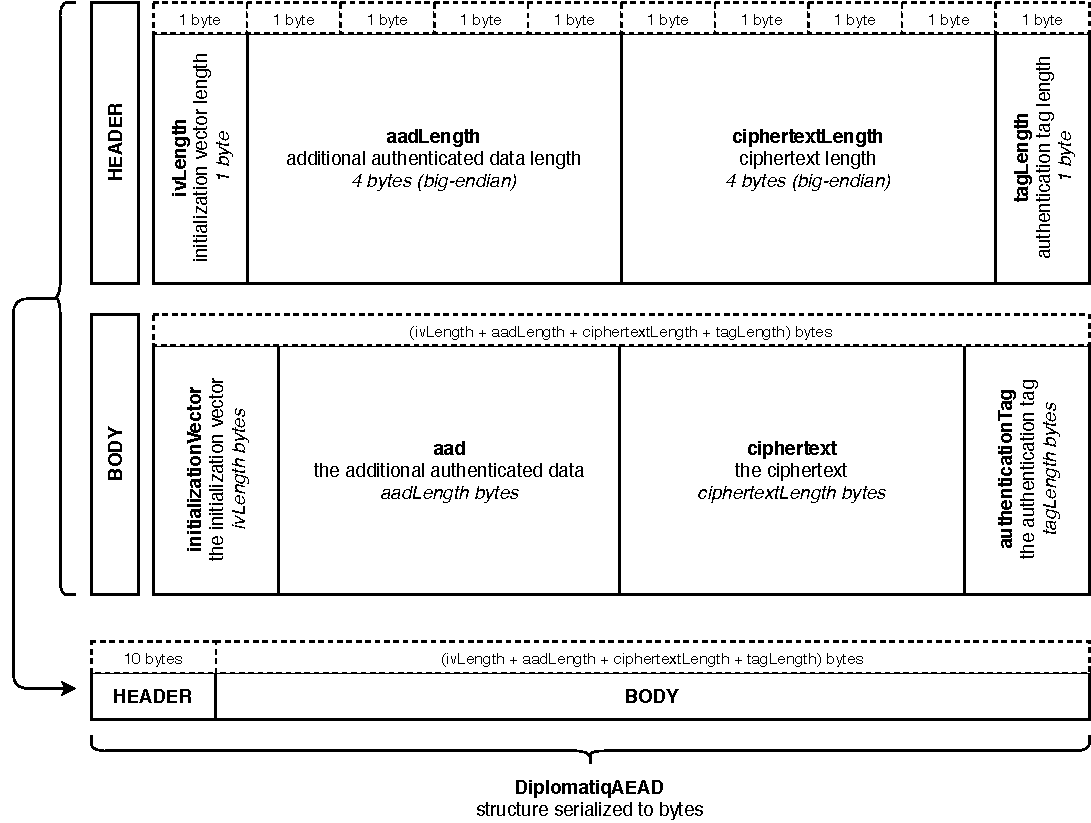
\includegraphics[width=\textwidth]{figures/aead.pdf}
    \caption{The structure of DiplomatiqAEAD serialized to bytes}
    \label{fig:aead}
\end{figure}

\section{Applied web platform security measures}

\subsection{Cross-Site Scripting (XSS)}

Cross-Site Scripting (XSS) attacks are a type of code injection, in which malicious scripts are injected into otherwise benign and trusted websites. XSS attacks occur when an attacker uses a web application to send malicious code, generally in the form of a browser side script, to an end user. Flaws that allow these attacks to succeed are quite widespread and occur anywhere a web application uses input from a user within the output it generates without validating or encoding it~\cite{owasp-xss}. Although in most modern browsers, a strong Content Security Policy ruleset disabling inline JavaScript can mitigate XSS, in older browsers the \lstinline{X-XSS-Protection} header can be used to instruct the browser to prevent rendering the page if an XSS attack is detected. Diplomatiq includes the \lstinline{X-XSS-Protection} header into its responses. The Angular framework also implements strong XSS mitigation measures: as long as their built-in filtering is used to display dynamic data in the browser, the application is protected. Diplomatiq uses Angular's built-in filtering.

\subsection{Content Security Policy (CSP)}

The Content Security Policy browser mechanism allows websites and web applications to specify what kind of resourcs (e.g. images, stylesheet files, script files, font files) can be loaded within the context of the application, and what kind of domains can the application connect to via network calls. This can protect against XSS attacks, and can also protect against performing unauthorized API calls. Diplomatiq applies a very strict Content Security Policy ruleset, which restricts everything by default, and only allows loading images, script files, stylesheet files, and font files from the application's very own domain name. Inline scripts are not allowed, meaning the application is safe against XSS attacks. Diplomatiq's policy allows connecting the front end application to \emph{api.diplomatiq.org} only.

\subsection{Cross-Origin Resource Sharing (CORS)}

By default, web browsers enforce the same-origin policy, meaning a web application running on a given domain can not initiate network requests to another domain. The Cross-Origin Resource Sharing mechanism instructs the browser to allow an application running on a certain origin to connect to a domain different than its origin. CORS settings are communicated to browsers via additional HTTP headers, specifying the origins which are allowed to connect to the domain which issued the headers. The Diplomatiq back end application issues CORS headers, which authorizes the application running under \emph{app.diplomatiq.org} to connect to the back end. No other application is authorized other than Diplomatiq's front end application.

\subsection{Feature Policy}

The Feature Policy experimental mecahnism enables to deny the usage of browser features for a web application, such as the browser's geolocation API, camera API, vibrate API, full screen API, etc. Feature Policy settings are communicated to the browser via a \lstinline{Feature-Policy} header. Their Feature Policies being the strictest, Diplomatiq's applications are not authorized to use such browser APIs at all.

\subsection{Referrer Policy}

The Referrer Policy mechanism can mitigate threats associated with the \lstinline{Referer}\footnote{The \lstinline{Referer} header is a misspelling of word \textquote{referrer}.} header. The \lstinline{Referer} header contains the URL of the page which the user visited before navigated to the current page. Referrer Policy settings are communicated to the browser via the \lstinline{Referrer-Policy} header. Their Referrer Policies being the strictest, Diplomatiq's applications omit the \lstinline{Referer} header entirely.

\subsection{Preventing click-jacking}

Click-jacking is a type of attacks where a page is embedded into another page via an \lstinline{<frame>} or \lstinline{<iframe>} element, and the user's clicks are hijacked to perform additional interactions on other web sites. Click-jacking can be prevented by instructing browsers not to allow embedding an application. Although Diplomatiq's restrictive Content Security Policy protects against this in modern browsers, in older browsers the \lstinline{X-Frame-Options} header should be set to \lstinline{DENY}. Diplomatiq's applications set this header accordingly as well.

\section{Authentication and authorization}

according to NIST https://nvlpubs.nist.gov/nistpubs/SpecialPublications/NIST.SP.800-63-3.pdf, multifactor authentication is necessary

oawsp top 10. listán 2. broken auth https://owasp.org/www-project-top-ten/

authentication why not oauth/openid/standard megoldások?

    1. signed requests and authentication

    2. session levels

    3. SRP

    4. cryptography

aláíráshoz az amazonos aláírásból indultam ki.

device container

\begin{figure}[!htb]
    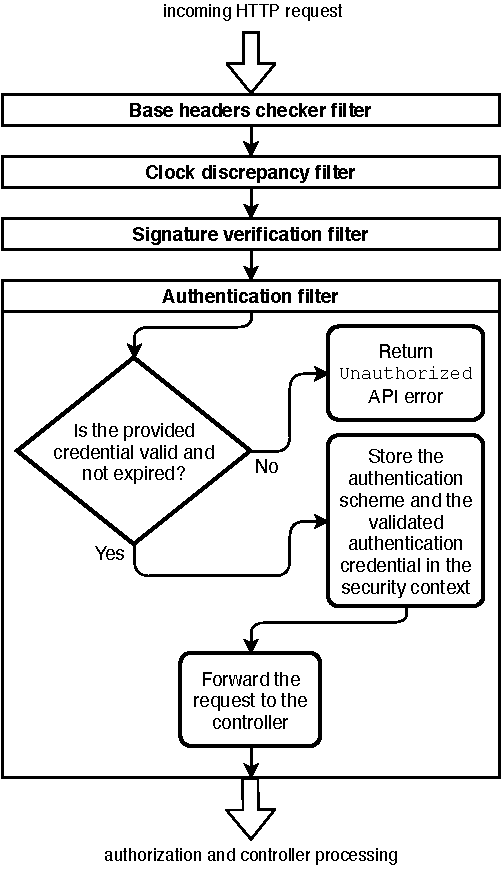
\includegraphics[width=\textwidth]{figures/authentication-filter.pdf}
    \caption{The authentication filter}
    \label{fig:authentication-filter}
\end{figure}

\begin{figure}[!htb]
    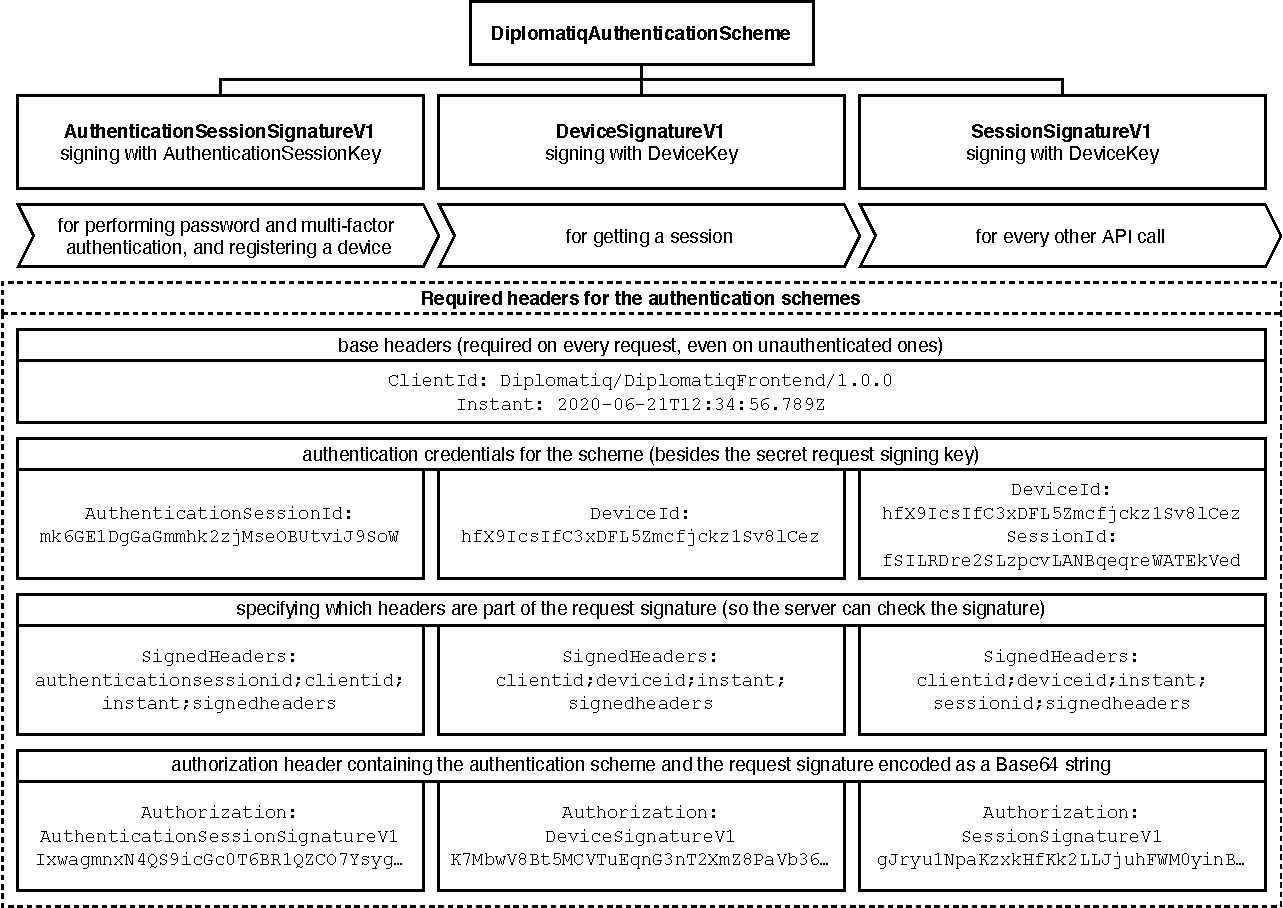
\includegraphics[width=\textwidth]{figures/authentication-schemes.pdf}
    \caption{A summary of Diplomatiq's authentication schemes}
    \label{fig:authentication-schemes}
\end{figure}

\begin{figure}[!htb]
    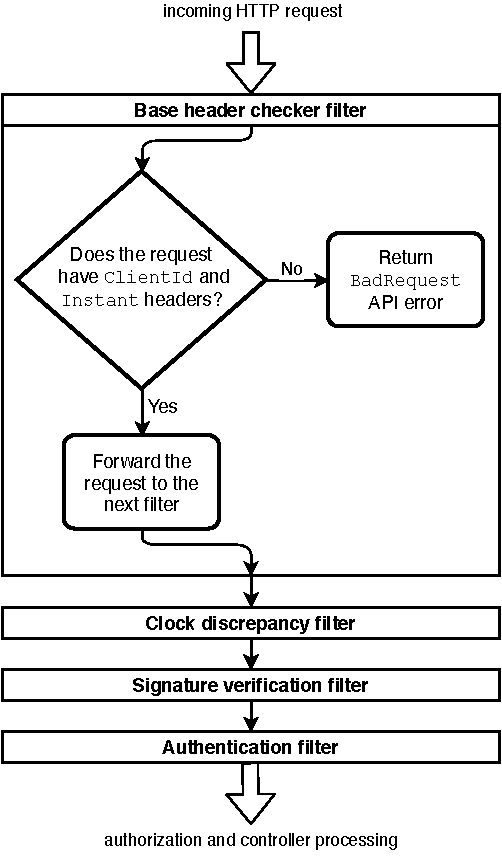
\includegraphics[width=\textwidth]{figures/base-headers-checker-filter.pdf}
    \caption{The base headers checker filter}
    \label{fig:base-headers-checker-filter}
\end{figure}

\begin{figure}[!htb]
    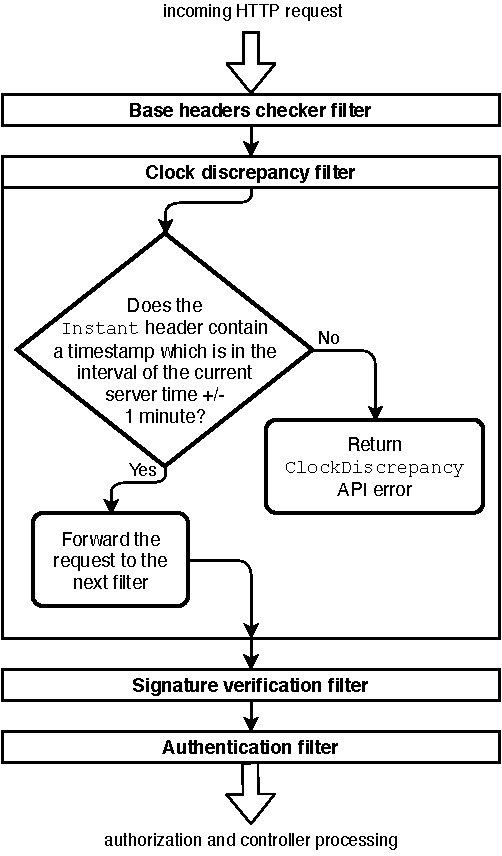
\includegraphics[width=\textwidth]{figures/clock-discrepancy-filter.pdf}
    \caption{The clock discrepancy filter}
    \label{fig:clock-discrepancy-filter}
\end{figure}

\begin{figure}[!htb]
    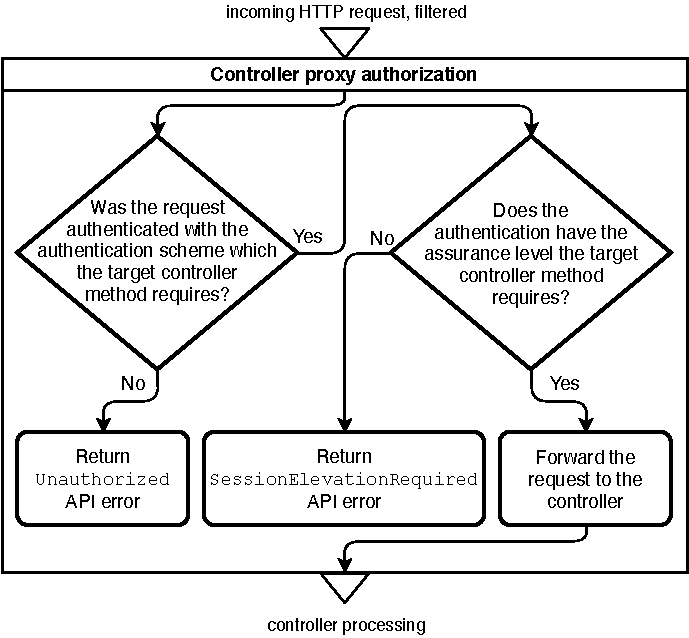
\includegraphics[width=\textwidth]{figures/controller-authorization.pdf}
    \caption{A summary of controller authorization}
    \label{fig:controller-authorization}
\end{figure}

\begin{figure}[!htb]
    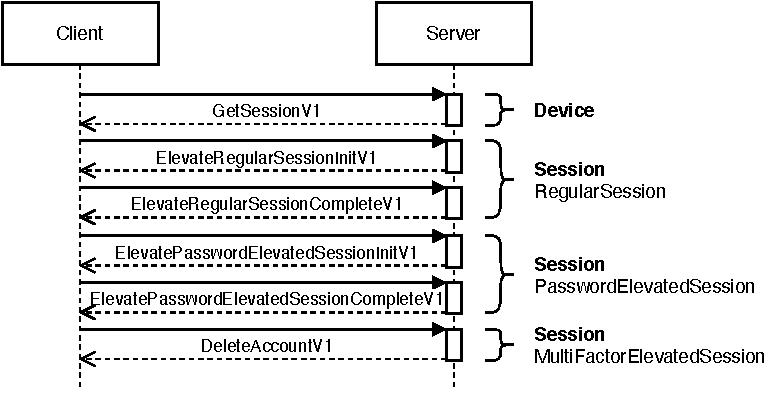
\includegraphics[width=\textwidth]{figures/elevate-to-mfa-session.pdf}
    \caption{Server calls for elevating a session to multi-factor level}
    \label{fig:elevate-to-mfa-session}
\end{figure}

\begin{figure}[!htb]
    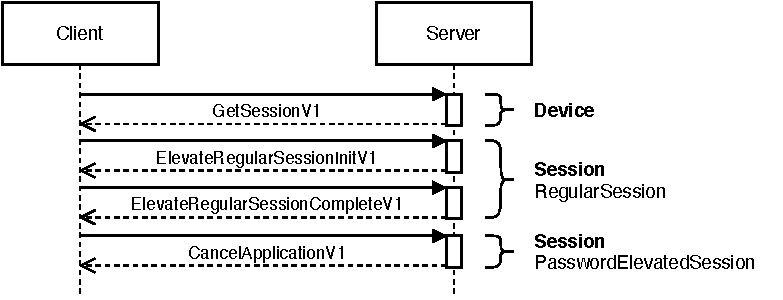
\includegraphics[width=\textwidth]{figures/elevate-to-password-session.pdf}
    \caption{Server calls for elevating a session to password level}
    \label{fig:elevate-to-password-session}
\end{figure}

\begin{figure}[!htb]
    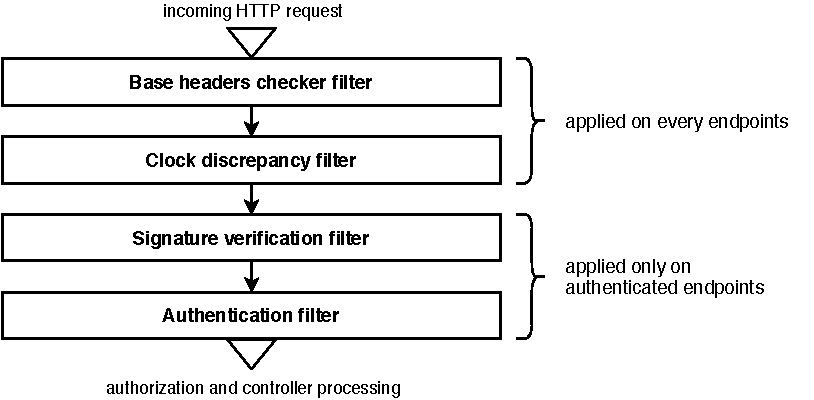
\includegraphics[width=\textwidth]{figures/request-filters.pdf}
    \caption{A summary of the back end application's request filters}
    \label{fig:request-filters}
\end{figure}

\begin{figure}[!htb]
    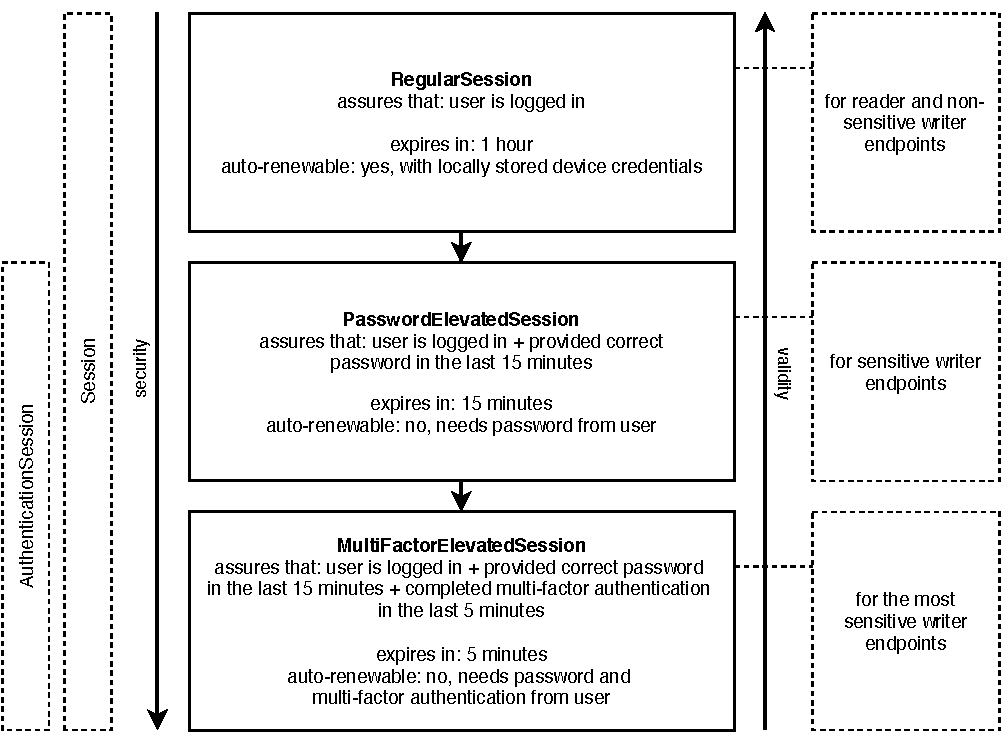
\includegraphics[width=\textwidth]{figures/session-assurance-levels.pdf}
    \caption{Diplomatiq's session assurance levels}
    \label{fig:session-assurance-levels}
\end{figure}

\begin{figure}[!htb]
    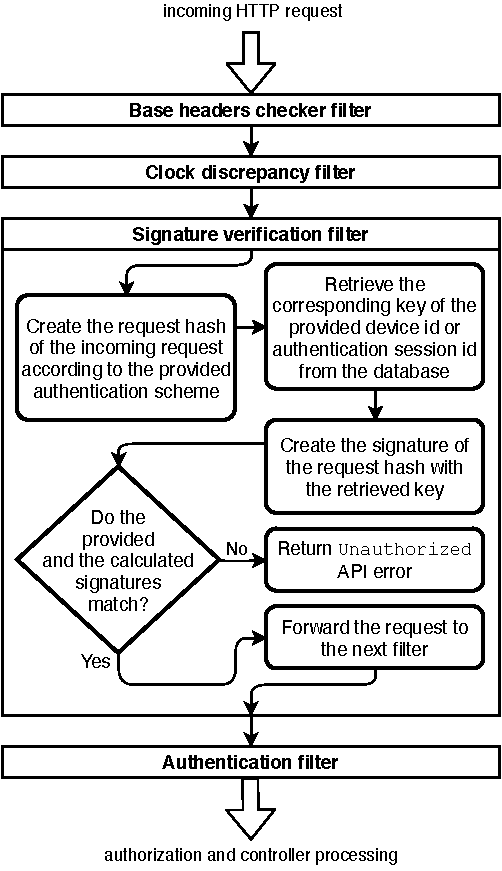
\includegraphics[width=\textwidth]{figures/signature-verification-filter.pdf}
    \caption{The signature verification filter}
    \label{fig:signature-verification-filter}
\end{figure}

\section{Encrypting sensitive data in the database}

encrypted db values, key versioning to avoid birthday problem

\section{Other security measures}

nem adunk ki a userről adatot (hogy létezik-e ilyen mailcímű user, stb)

security.txt

\chapter{Monetization and business model}
\label{chapter:business}

\chapter{Conclusion and future work}
\label{chapter:conclusion}

\chapter*{Acknowledgements}
\phantomsection
\addcontentsline{toc}{chapter}{Acknowledgements}
\thispagestyle{plain}

Asztalos Márk, Hidvégi Roland, Noémi, Anyu, Apa, nagyi, Peti, Isti, Marussy Kristóf, család, barátok.

%%% Local Variables:
%%% mode: latex
%%% TeX-master: "main"
%%% End:


\printbibliography

\appendix
\chapter*{Appendix}
\phantomsection
\addcontentsline{toc}{chapter}{Appendix}
\renewcommand{\thesection}{\Alph{section}}

\section{Tables}

\subsection{Email addresses configured for diplomatiq.org}

\begin{table}[!htb]
    \centering
    \begin{tabular}{l|l|l}
        \toprule
        \textbf{Email address}      & \textbf{Usage}            & \textbf{Notes} \\
        \midrule
        billing@diplomatiq.org     & sending \& receiving      & for billing-related notifications \\
        ceo@diplomatiq.org         & sending \& receiving      & for communicating as the CEO \\
        conduct@diplomatiq.org     & receiving                 & for Code of Conduct violations \\
        github@diplomatiq.org      & sending \& receiving      & for the GitHub service \\
        info@diplomatiq.org        & receiving                 & for personal inquiries \\
        npm@diplomatiq.org         & sending \& receiving      & for Microsoft services \\
        npm@diplomatiq.org         & sending \& receiving      & for the NPM service \\
        security@diplomatiq.org    & receiving                 & for security inquiries \\
        soma.lucz@diplomatiq.org   & sending \& receiving      & for communicating as myself \\
        team@diplomatiq.org        & sending                   & for sending transactional email \\
        \bottomrule
    \end{tabular}
\end{table}

\newpage

\section{Figures}

\subsection{Server calls for elevating a session to password level}

\begin{figure}[!htb]
    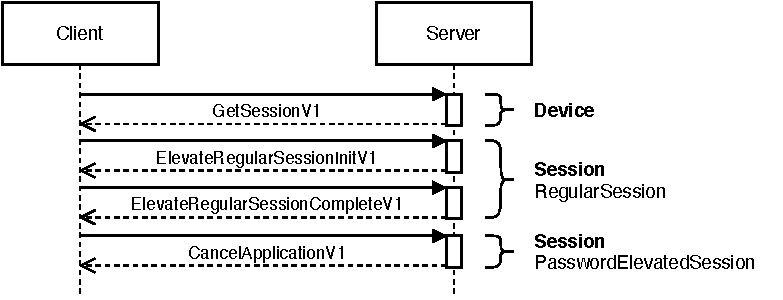
\includegraphics[width=\textwidth]{figures/elevate-to-password-session.pdf}
\end{figure}

\subsection{Server calls for elevating a session to password level}

\begin{figure}[!htb]
    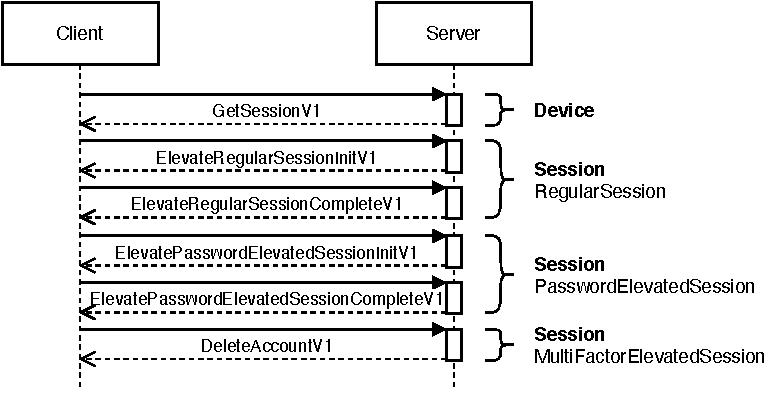
\includegraphics[width=\textwidth]{figures/elevate-to-mfa-session.pdf}
\end{figure}


\label{page:last}

\end{document}

%%% Local Variables:
%%% mode: latex
%%% TeX-master: nil
%%% End:
